\documentclass[
	12pt,
	a4paper,
	bibtotoc,
	cleardoubleempty, 
	idxtotoc,
	ngerman,
	openright
	final,
	listof=nochaptergap,
	]{scrbook}

\usepackage[T1]{fontenc}
\usepackage[utf8]{inputenc}
\usepackage[ngerman]{babel}

% ##################################################
% Unterstuetzung fuer die deutsche Sprache
% ##################################################
\usepackage{ngerman}
\usepackage[ngerman]{babel}

% ##################################################
% Dokumentvariablen
% ##################################################

% Persoenliche Daten
\newcommand{\docNachname}{}
\newcommand{\docVorname}{}
\newcommand{\docStrasse}{}
\newcommand{\docOrt}{Furtwangen}
\newcommand{\docPlz}{}
\newcommand{\docEmail}{}
\newcommand{\docMatrikelnummer}{}

% Dokumentdaten
\newcommand{\docTitle}{PIPCO}
%\newcommand{\docUntertitle}{} % Kein Untertitel
\newcommand{\docUntertitle}{Private IP Camera Observation}
% Arten der Arbeit: Bachelorthesis, Masterthesis, Seminararbeit, Diplomarbeit
\newcommand{\docArtDerArbeit}{Projektdokumentation}
%Studiengaenge: Allgemeine Informatik Bachelor, Computer Networking Bachelor,
% Software-Produktmanagement Bachelor, Advanced Computer Scinece Master
\newcommand{\docStudiengang}{AIN}
\newcommand{\docAbgabedatum}{13.01.2019}
\newcommand{\docErsterReferent}{Prof. Dr. Elmar Cochlovius}
%\newcommand{\docZweiterReferent}{-} % Wenn es nur einen Betreuer gibt
%\newcommand{\docZweiterReferent}{ZWEITER REFERENT}

% ##################################################
% Allgemeine Pakete
% ##################################################

% Abbildungen einbinden
\usepackage{graphicx}

% Zusaetsliche Sonderzeichen
\usepackage{dingbat}

% Farben
\usepackage{color}
\usepackage[usenames,dvipsnames,svgnames,table]{xcolor}

% Maskierung von URLs und Dateipfaden
\usepackage[hyphens]{url}

% Deutsche Anfuehrungszeichen
\usepackage[babel, german=quotes]{csquotes}

% Pakte zur Index-Erstellung (Schlagwortverzeichnis)
\usepackage{index}
\makeindex

% Ipsum Lorem
% Paket wird nur für das Beispiel gebraucht und kann gelöscht werden
\usepackage{lipsum}

% ##################################################
% Seitenformatierung
% ##################################################
\usepackage[
	portrait,
	bindingoffset=1.5cm,
	inner=2.5cm,
	outer=2.5cm,
	top=3cm,
	bottom=2cm,
	%includeheadfoot
	]{geometry}

% ##################################################
% Kopf- und Fusszeile
% ##################################################

\usepackage{fancyhdr}

\pagestyle{fancy}
\fancyhf{}
\fancyhead[EL,OR]{\sffamily\thepage}
\fancyhead[ER,OL]{\sffamily\leftmark}

\fancypagestyle{headings}{}

\fancypagestyle{plain}{}

\fancypagestyle{empty}{
  \fancyhf{}
  \renewcommand{\headrulewidth}{0pt}
}

%Kein "Kapitel # NAME" in der Kopfzeile
\renewcommand{\chaptermark}[1]{
	\markboth{#1}{}
   	\markboth{\thechapter.\ #1}{}
}

% ##################################################
% Schriften
% ##################################################

% Stdandardschrift festlegen
\renewcommand{\familydefault}{\sfdefault}

% Standard Zeilenabstand: 1,5 zeilig
\usepackage{setspace}
\onehalfspacing 

% Schriftgroessen festlegen
\addtokomafont{chapter}{\sffamily\large\bfseries} 
\addtokomafont{section}{\sffamily\normalsize\bfseries} 
\addtokomafont{subsection}{\sffamily\normalsize\mdseries} 
\addtokomafont{caption}{\sffamily\normalsize\mdseries} 

% ##################################################
% Inhaltsverzeichnis / Allgemeine Verzeichniseinstellungen
% ##################################################

\usepackage{tocloft}

% Punkte auch bei Kapiteln
\renewcommand{\cftchapdotsep}{3}
\renewcommand{\cftdotsep}{3}

% Schriftart und -groesse im Inhaltsverzeichnis anpassen
\renewcommand{\cftchapfont}{\sffamily\normalsize}
\renewcommand{\cftsecfont}{\sffamily\normalsize}
\renewcommand{\cftsubsecfont}{\sffamily\normalsize}
\renewcommand{\cftchappagefont}{\sffamily\normalsize}
\renewcommand{\cftsecpagefont}{\sffamily\normalsize}
\renewcommand{\cftsubsecpagefont}{\sffamily\normalsize}

%Zeilenabstand in den Verzeichnissen einstellen
\setlength{\cftparskip}{.5\baselineskip}
\setlength{\cftbeforechapskip}{.1\baselineskip}

% ##################################################
% Abbildungsverzeichnis und Abbildungen
% ##################################################

\usepackage{caption}

\usepackage{wrapfig}

% Nummerierung von Abbildungen
\renewcommand{\thefigure}{\arabic{figure}}
\usepackage{chngcntr}
\counterwithout{figure}{chapter}

% Abbildungsverzeichnis anpassen
\renewcommand{\cftfigpresnum}{Abbildung }
\renewcommand{\cftfigaftersnum}{:}

% Breite des Nummerierungsbereiches [Abbildung 1:]
\newlength{\figureLength}
\settowidth{\figureLength}{\bfseries\cftfigpresnum\cftfigaftersnum}
\setlength{\cftfignumwidth}{\figureLength}
\setlength{\cftfigindent}{0cm}

% Schriftart anpassen
\renewcommand\cftfigfont{\sffamily}
\renewcommand\cftfigpagefont{\sffamily}

% ##################################################
% Tabellenverzeichnis und Tabellen
% ##################################################

% Nummerierung von Tabellen
\renewcommand{\thetable}{\arabic{table}}
\counterwithout{table}{chapter}

% Tabellenverzeichnis anpassen
\renewcommand{\cfttabpresnum}{Tabelle }
\renewcommand{\cfttabaftersnum}{:}

% Breite des Nummerierungsbereiches [Abbildung 1:]
\newlength{\tableLength}
\settowidth{\tableLength}{\bfseries\cfttabpresnum\cfttabaftersnum}
\setlength{\cfttabnumwidth}{\tableLength}
\setlength{\cfttabindent}{0cm}

%Schriftart anpassen
\renewcommand\cfttabfont{\sffamily}
\renewcommand\cfttabpagefont{\sffamily}

% Unterdrueckung von vertikalen Linien
\usepackage{booktabs}

% ##################################################
% Listings (Quellcode)
% ##################################################

\usepackage{listings}
\lstset{
	language=java,
	backgroundcolor=\color{white},
	breaklines=true,
	prebreak={\carriagereturn},
 	breakautoindent=true,
 	numbers=left,
 	numberstyle=\tiny,
 	stepnumber=2,
 	numbersep=5pt,
 	keywordstyle=\color{blue},
   	commentstyle=\color{green},   
   	stringstyle=\color{gray}
}
  	
% ##################################################
% Theoreme
% ##################################################
  	
% Umgebung fuer Beispiele
\newtheorem{beispiel}{Beispiel}

% Umgebung fuer These
\newtheorem{these}{These}

% Umgebung fuer Definitionen
\newtheorem{definition}{Definition}
  	
% ##################################################
% Literaturverzeichnis
% ##################################################

\usepackage{bibgerm}

% ##################################################
% Abkuerzungsverzeichnis
% ##################################################

\usepackage[printonlyused]{acronym}

% ##################################################
% PDF / Dokumenteninternelinks
% ##################################################

\usepackage[
	colorlinks=false,
   	linkcolor=black,
   	citecolor=black,
  	filecolor=black,
	urlcolor=black,
    bookmarks=true,
    bookmarksopen=true,
    bookmarksopenlevel=3,
    bookmarksnumbered,
    plainpages=false,
    pdfpagelabels=true,
    hyperfootnotes,
    pdftitle ={\docTitle},
    pdfauthor={\docVorname~\docNachname},
    pdfcreator={\docVorname~\docNachname}]{hyperref}

\begin{document}

\setcounter{secnumdepth}{3}

% Titelblatt
\begin{titlepage}
\pagestyle{empty}

% ##################################################
% HFU-Logo einbinden
% ##################################################
\begin{flushright}
\begin{figure}[ht]
\flushright

\includegraphics[height=3cm]{content/pictures/hfu.jpg}
\end{figure}
\end{flushright}

% ##################################################
% Titel
% ##################################################
\begin{center}
{\fontsize{18}{22} \selectfont \docArtDerArbeit}\\[5mm]
{\fontsize{18}{22} \selectfont im Studiengang} \\[5mm]
{\fontsize{18}{22} \selectfont \docStudiengang}\\
\vspace{1cm}
\begin{onehalfspace}
{\fontsize{22}{26} \selectfont \textbf{\docTitle}}\\[5mm]
{\fontsize{18}{22} \selectfont \docUntertitle}


\end{onehalfspace}
\end{center}

% ##################################################
% Zusatzinformationen
% ##################################################
\vfill
\begin{center}
\begin{tabular}{lcl}
Referent  		&:& \docErsterReferent 	\\ \\
Vorgelegt am 	&:& \docAbgabedatum 	\\ \\
%Vorgelegt von 	&:& \docVorname~\docNachname\\
%				& & Matrikelnummer: \docMatrikelnummer\\
%				& & \docStrasse,~\docPlz~\docOrt	\\
%				& & \docEmail			
\end{tabular}
\end{center}
\end{titlepage}
\cleardoubleemptypage

\frontmatter


% Abstract
\chapter*{Abstract\markboth{Abstract}{}}
\addcontentsline{toc}{chapter}{Abstract}

[Englisches Abstract (100-120 Worte)]

[Deutsches Abstract (100-120 Worte)]
\cleardoubleemptypage

% Inhaltsverzeichnis
\tableofcontents
\addcontentsline{toc}{chapter}{Inhaltsverzeichnis}
\cleardoubleemptypage

% Abbildungsverzeichnis einbinden und ins Inhaltsverzeichnis
% WORKAROUND: tocloft und KOMA funktionieren zusammen nicht
% korrekt\phantomsection
\addcontentsline{toc}{chapter}{\listfigurename} 
\listoffigures
\cleardoubleemptypage

% Tabellenverzeichnis einbinden und ins Inhaltsverzeichnis
% WORKAROUND: tocloft und KOMA funktionieren zusammen nicht
% korrekt\phantomsection
\phantomsection
\addcontentsline{toc}{chapter}{\listtablename}
\listoftables
\cleardoubleemptypage

% Abkürzungsverzeichnis
\chapter*{Abkürzungsverzeichnis\markboth{Abkürzungsverzeichnis}{}}
\addcontentsline{toc}{chapter}{Abkürzungsverzeichnis}

\begin{acronym}
\acro{HFU}{Hochschule Furtwangen University}
\acro{IP}{Internet Protocol}
\acro{PC}{Personal Computer}
\acro{CLI}{Command Line Interface}
\acro{URL}{Uniform Resource Locator}
\acro{MIT}{Massachusetts Institute of Technology}
\acro{CSS}{Cascading Style Sheets}
\acro{HTML}{Hyper Text Markup Language}
\end{acronym}

\mainmatter

\chapter{Einleitung}
\section{Rahmenbedinungen}
Dieses Projekt stellt das Semesterprojekt von vier Studenten des Studienganges Allgemeine Informatik der Hochschule in Furtwangen dar. Es handelt sich dabei um das zweite Semesterprojekt, welches im sechsten Semester stattfindet. 

Ziel des Projektes ist es, eine Software zur Überwachtung mittels \acs{IP}-Kamera zu implementieren, wobei die genutzte Hardware austauschbar bleiben soll. Die Anwendung soll die Fähigkeit besitzen, Bewegungen im Kameralivestream zu detektieren und zuvor hinterlegte Nutzer per E-Mail über die erkannten Bewegungen in Kenntnis zu setzen. Außerdem sollen Aufnahmen dieser Bewegungen erstellt und für den Endanwender einsehbar hinterlegt werden. Neben diversen Einstellungsmöglichkeiten für den Nutzer, wie zum Beispiel für die Sensitivität der Bewegungserkennung oder einer maximalen Anzahl an gespeicherten Aufnahmen soll die Anwendung über eine nutzerfreundliche Weboberfläche mit Login-Maske verfügen.

Unter der Betreuung von Prof. Dr. Elmar Cochlovius und Judith Jakob wurde das Projekt weitestgehend selbstorganisiert durchgeführt. Ein für Testzwecke erforderlicher Hardware-Aufbau konnte im Smart-Home-Labor am Campus in Furtwangen genutzt werden. Dort waren auch ähnliche Lösungen von kommerziellen Anbietern vorhanden, welche während dem Projekt als Referenzen gedient haben.
\chapter{Planung}
\section{Rollenverteilung}
\section{Anforderungen}
\section{Meilensteine}
\section{Architektur}
Bei dem ersten Treffen mit dem 'Kunden' wurde von uns eine Software zur Überwachung eines Raumes mithilfe einer herkömmlichen IP-Kamera gewünscht.
Da hierfür auch eine Möglichkeit zur Interaktion mit dem System gegeben sein sollte, entschieden wir uns für eine Webseite, mit welcher
der Videofeed sichtbar und Einstellungen vorgenommen werden sollten. Da die Software im Gegensatz zu anderen kommerziellen Produkten im lokalen Netz bleiben sollte,
spielte die Sicherheit keine große Rolle.\\
Die Architektur sollte die Aufteilung der Schichten wie Logik, Datenhaltung sowie die Präsentation durch den Webserver darstellen.
Hierfür wurde zuerst Abbildung \ref{img:architecture-sketch} erstellt.\\\\
\begin{figure}[h]
	\centering
	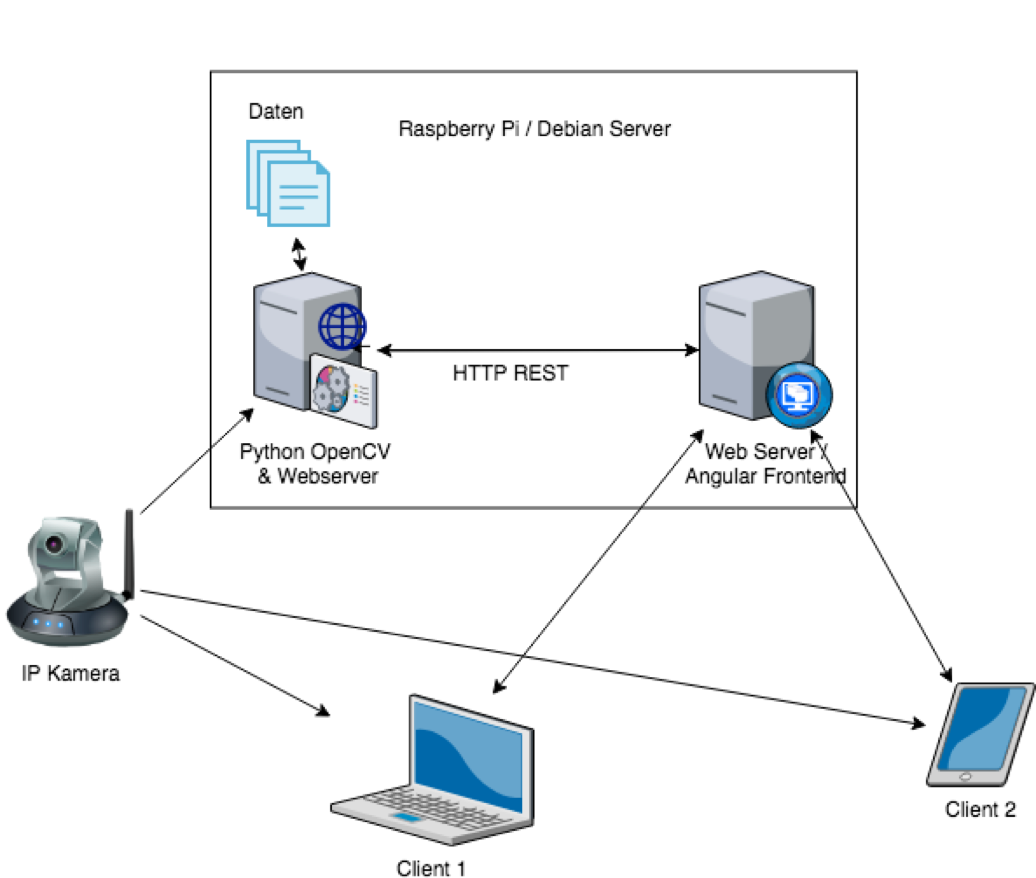
\includegraphics[height=10cm]{content/pictures/architecture-sketch.png}
	\caption{Erste Planung der Architektur}
	\label{img:architecture-sketch}
\end{figure}
Da der Architekt im Gebiet der Webtechnologien kaum Erfahrung hatte, entschieden die verantwortlichen Entwickler sich selbst für Angular und sprachen sich bei
der Entwicklung ab. Lediglich REST wurde für die Kommunikation zwischen Frontend und Backend definiert. 
Um die Aufteilung der Klassen und Kommunikation innerhalb des Backends darzustellen wurde ein grobes Klassendiagramm erstellt (Abbildung \ref{img:backend-classdiagramm}).\\\\
\begin{figure}[]
	\centering
	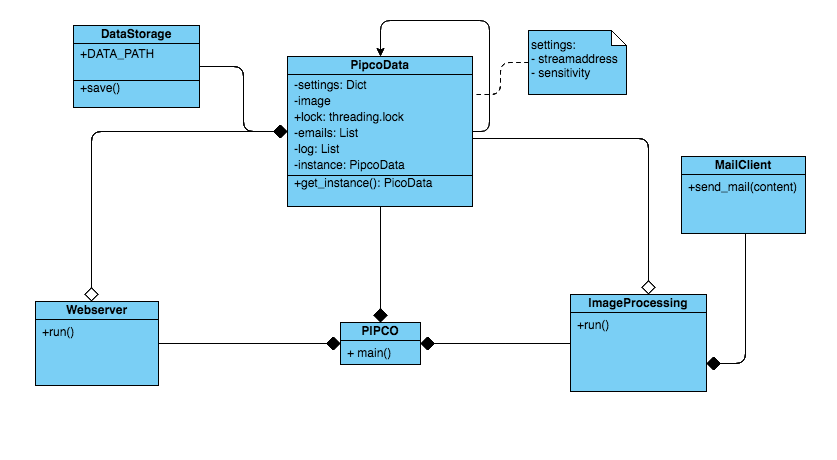
\includegraphics[width=\textwidth]{content/pictures/classdiagramm.png}
	\caption{Klassendiagramm Aufbau des Backends}
	\label{img:backend-classdiagramm}
\end{figure}
Für die Unabhängige Entwicklung der Kommunikation von Frontend und Backend wurde eine Liste mit den notwendigen REST-Nachrichten erstellt (Tabelle \ref{table:kommunikation}).\\\\
\begin{table}[]
	\centering
	\caption{Kommunikation Backend und Frontend}
	\label{table:kommunikation}
	\resizebox{\textwidth}{!}{\begin{tabular}{llll}
		\textbf{Type} & \textbf{address}                                                             & \textbf{keys}                                                                                                                                                                                                                                          & \textbf{returns}           \\
		POST          & /login                                                                       & user, password                                                                                                                                                                                                                                         & OK / Error 403             \\
		GET           & /videostream                                                                 &                                                                                                                                                                                                                                                        & mjpeg stream               \\
		GET           & /logs/\textless{}page\_no\textgreater{}/\textless{}batch\_size\textgreater{} &                                                                                                                                                                                                                                                        & list with logs             \\
		DELETE        & /log/\textless{}log\_id\textgreater{}                                        &                                                                                                                                                                                                                                                        & id / Error 403             \\
		POST          & /mail                                                                        &                                                                                                                                                                                                                                                        & id / Error 403             \\
		GET           & /mails                                                                       &                                                                                                                                                                                                                                                        & list of mail addresses     \\
		DELETE        & /mail/\textless{}mail\_id\textgreater{}                                      &                                                                                                                                                                                                                                                        & id / Error 403             \\
		PUT           & /mail/\textless{}mail\_id\textgreater{}                                      &                                                                                                                                                                                                                                                        & notify status / Error 403  \\
		POST          & /config                                                                      & \multirow{4}{*}{\begin{tabular}[c]{@{}l@{}}sensitivity(float), streamaddress,brightness (float),\\ contrast (float), log\_enabled(bool),\\ global\_notify(bool), cliplength (int in seconds),\\ max\_logs (int),max\_storage (int in MB)\end{tabular}} & changed values / Error 403 \\
		&                                                                              &                                                                                                                                                                                                                                                        &                            \\
		&                                                                              &                                                                                                                                                                                                                                                        &                            \\
		&                                                                              &                                                                                                                                                                                                                                                        &                            \\
		GET           & config                                                                       &                                                                                                                                                                                                                                                        & config                     \\
		GET           & /recording/\textless{}filename\textgreater{}                                 &                                                                                                                                                                                                                                                        & videofile                  \\
		GET           & /backup                                                                      &                                                                                                                                                                                                                                                        & backup.zip                 \\
		&                                                                              &                                                                                                                                                                                                                                                        &                           
	\end{tabular}}
\end{table}
Während der Entwicklung stellte sich heraus, dass der Aufwand für die Implementierung der bidirektionalen Kommunikation zwischen Frontend und Backend zu hoch ist, weshalb wir uns dazu entschieden die Daten direkt vom Backend zu holen und die Logs mithilfe von Polling aktuell zu halten.
Eine weitere Änderung war die Kamera, welche lediglich vom Backend angefragt wird. Der Client sollte sich ausschließlich die Bilder, mit eingezeichneten Bewegungen holen.
Hierdurch änderte sich die Architektur wie in Abbildung \ref{img:architecture-change} zu sehen.\\

Um den Ablauf besser nachvollziehen zu können wurde desweiteren ein Sequenzdiagramm erstellt (Abbildung \ref{img:sequencediagram}).

\begin{figure}[]
	\centering
	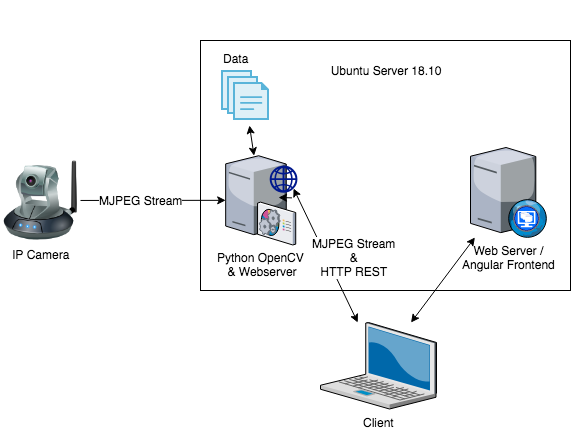
\includegraphics[width=\textwidth]{content/pictures/architecture-change.png}
	\caption{Klassendiagramm: Direkter Zugriff auf das Backend}
	\label{img:architecture-change}
\end{figure}

\begin{figure}[]
	\centering
	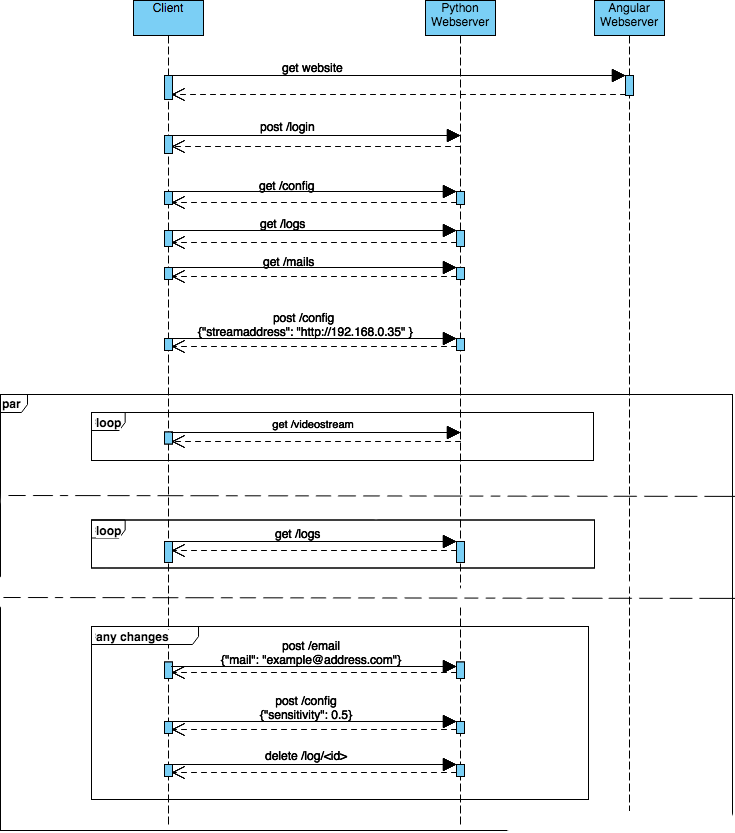
\includegraphics[width=\textwidth]{content/pictures/sequencediagram.png}
	\caption{Ablauf Login und Änderungen}
	\label{img:sequencediagram}
\end{figure}
\chapter{Front-End}\label{frontendchapter}
Da zwei der vier Projektteilnehmer bereits im Praxissemester Erfahrungen damit gesammelt haben, viel unsere Wahl bei den Technologien für unser Front-End auf Angular. Auf diese Weise konnten wir produktiver arbeiten und deutlich übersichtlicheren Code produzieren. Grundlegende Informationen rund um Angular sowie ein Tutorial zur Entwicklung mit Angular gibt es unter \href{https://angular.io/}{https://angular.io/}, der offiziellen Website zum Framework.

\section{Angular}
Angular ist ein unter der sehr freizügigen \acs{MIT}-Lizenz verfügbares, auf TypeScript basierendes Front-End-Framework für Webanwendungen, wobei die Entwicklung dieser Software von Google geleitet wird. Dieses Framework ist grundsätzlich Client-seitig, was bedeutet, dass unter anderem Darstellung sowie Strukturierung von Inhalten beim Anwender und nicht auf der Host-Maschine berechnet werden. Eine Kommunikation mit dem Server findet demnach nur dann statt, wenn neue Inhalte abgerufen werden, oder wenn ein weiterer Datenaustausch vom Entwickler vorgesehen ist. Das hat den Vorteil, dass die Kapazitäten des Servers geschont werden.

Neben den offensichtlichen Vorteilen eines Frameworks, wie zum Beispiel dem Steigern der Produktivität des Entwicklers durch die Abstraktion häufig auftretender Problemstellungen, bietet Angular den Vorteil einer komponentenorientierten Herangehensweise bei der Strukturierung von damit erstellten Webanwendungen. Durch diese Unterteilung semantisch zusammengehöriger Codebausteine wird eine ansonsten komplexe Anwendung übersichtlicher und damit wartbarer. Zudem können solche Komponenten aufgrund ihrer Kapselung deutlich einfacher getestet oder auch an anderer Stelle wiederverwendet werden. Einer der Hauptgründe dafür, dass in Angular eine so strikte Trennung einzelner Komponenten überhaupt möglich ist, stellt dabei die fundamentale Unterstützung von Dependency Injection dar.

Durch die Verwendung der JavaScript-Spracherweiterung TypeScript als Primärsprache des Frameworks profitieren Angular-Entwickler zudem von den Vorteilen der Objektorientierung. Zusätzlich wurde in TypeScript eine statische Typisierung für Variablen eingeführt, was dem Entwickler dabei unterstützt, dahingehende Fehler bereits beim Bauen der Anwendung aufzudecken. \cite{OWA18}

\subsection{Begriffe}
Um Neulingen in Sachen Angular einen leichteren Einstieg zu bereiten, werden im folgenden einige Kernbegriffe im Bezug auf unser Projekt geschildert. Am besten sollte jedoch die Einführung auf der offiziellen Seite zu Angular unter \href{https://angular.io/}{https://angular.io/} bearbeitet werden.

\subsubsection{Components}
Eine Angular-Component spiegelt in der Regel ein beliebig kleines Element in der Oberfläche einer Website dar. Eine Angular-Weboberfläche besteht ausschließlich aus einzelnen Components. Jede Component umfasst im Projekt drei Dateien, welche die Funktionalität der Komponente zur Verfügung stellen. Es gibt eine \acs{HTML}-Datei für die \acs{HTML}-Struktur, eine \acs{CSS}-Datei für das Styling sowie eine TypeScript-Datei für die Dynamik der Inhalte. \cite{OWA18}

\subsubsection{Services}
Angular-Services dienen in der Regel dazu, Daten mittels Http-Requests zu beschaffen und den Components der Anwendung zur Verfügung zu stellen. Dabei werden diese Services nicht direkt von den Komponenten erzeugt, sondern mittels dependency injection eingeschleust. Somit können unnötige Mehrfachinitialisierungen vermieden werden. Außerdem kann der Service damit zu einem für das Angular-Framework optimalen Zeitpunkt erzeugt werden. Ein Testen von Services nutzenden Komponenten kann durch das Verwenden der dependency injection ebenfalls besser umgesetzt werden, ohne auf die Implementierung der Services angewiesen zu sein, indem statt der eigentlichen Services Mock-Objekte injiziert werden. \cite{OWA18}

\subsubsection{Guards}
Die Seitennavigation kann bei Angular, so wie es auch in diesem Projekt der Fall ist, mittels \acs{URL}-Routen festgelegt werden. Sobald dann eine bestimmte \acs{URL} aufgerufen wird, wird eine vordefinierte Komponente angezeigt. Damit manche Routen nur unter bestimmten Umständen erreicht werden können, kann man Guards verwenden. Diese prüfen dann beim Aufrufen einer Route, ob die benötigten Bedingungen erfüllt sind und leitet den Nutzer nur dann wirklich weiter. In dieser Anwendung kommt beispielsweise für die Login-Funktionalität ein Guard zum Einsatz. \cite{OWA18}

\subsubsection{Module}
Angular-Module fassen eine inhaltlich sinnvoll vom Rest der Anwendung getrennte Sammlung von Programmelementen wie zum Beispiel Components oder Services zusammen. Services und Guards, welche innerhalb des Moduls mittels dependency injection erhalten können werden sollen, müssen im entsprechenden Modul angegeben werden. In dieser Anwendung gibt es neben dem Routing-Module (dazu später mehr) nur ein richtiges Module, welches Komponenten und Services bündelt, das App-Module. \cite{OWA18}

\section{Bausteine}
Hier werden in kurzer Form alle von uns erzeugten Bausteine des Front-Ends vorgestellt und erläutert.

\subsection{AppModule}
Die AppModule-Klasse stellt das einzige richtige Modul in unserer Anwendung dar. Hier werden alle Components deklariert, externe Module und damit deren Funktionalität importiert. Außerdem werden hier die für die dependency injection benötigten Services angegeben und damit bereitgestellt.

\subsection{RoutingModule}
\label{subsection_routingModule}
Der Sinn dieses Moduls besteht ausschließlich darin, das Routing der Anwendung zu realisieren. Hier werden alle \acs{URL}-Routen und die jeweiligen Komponenten als deren Gegenstück definiert. Durch das Verwenden von canActivate-Guards wird bei den Routen, die zur Hauptseite oder der Settings-Seite führen verhindert, dass diese ohne einen erfolgreichen Login erreicht werden können. Außerdem werden alle Routern, die nicht explizit von uns definiert wurden, durch die Nutzung einer Wildcard-Route auf die Login-Seite der Anwendung weitergeleitet.

\subsection{AppComponent}
Diese Komponente ist die Root-Komponente der Anwendung. In ihr wird keine Funktionalität implementiert, sondern lediglich der Grundaufbau der Webseite durch \acs{HTML}- sowie \acs{CSS}-Code definiert. Im \acs{HTML}-Teil ist dabei ein \glqq{}router-outlet\grqq{} genanntes Element auffällig. Dabei handelt es sich um einen Platzhalter für die jeweilige Komponente der aktuellen Route (siehe \ref{subsection_routingModule})

\subsection{HeaderComponent}
Die Header-Komponente stellt den Header der Weboberfläche dar und zeichnet sich vor allem dadurch aus, dass verschiedene Buttons je nach aktiver Router angezeigt werden. Neben einem permanenten Refresh-Button als Logo wird nur wenn der Anwender eingeloggt ist ein Logout-Button angezeigt, welcher den Anwender über den in \ref{subsection_authService} beschriebenen AuthService ausloggt und anschließend zur Login-Seite weiterleitet. Zudem gibt es je nachdem, ob sich der Nutzer auf der Haupt- oder Settings-Seite der Webanwendung befindet, einen Button der zu der jeweils anderen Seite führt.

\subsection{LoginComponent}
Hier wird der Aufbau der Login-Seite definiert. Zudem wird die Eingabe von Login-Daten und die Abwicklung des Login-Prozesses durch den in \ref{subsection_authService} beschriebenen AuthService geregelt. Bei erfolgreichem Login wird der Anwender auf die Hauptseite der Anwendung weitergeleitet und bei einem fehlgeschlagenem Login wird eine Fehlermeldung ausgegeben.

\subsection{MainPageComponent}
\label{subsection_mainPageComponent}
In dieser Komponente wird die Hauptseite der Anwendung beschrieben. Dabei geht es vor allem um den groben Aufbau und das Verhalten der Anwendung bei verschiedenen Bildschirmgrößen. Bei einer kleineren Auflösung rutschen die nebeneinander dargestellten Teilbereiche der Anwendung in eine Darstellung, bei der sie untereinander angeordnet werden. Das soll die Nutzung auf Geräten mit einer geringeren Auflösung oder einem anderen Bildformat verbessern. Die eigentlichen Inhalte der Hauptseite selbst, sind hierbei in anderen Komponenten definiert, welche hier lediglich eingebunden werden.

\subsection{RangeSliderComponent}
\label{subsection_rangeSliderComponent}
Die RangeSliderComponent nutzt die Funktionalitäten des \acs{HTML}-Input-Elementes des Typs Range und fügt dem ein ansprechendes Styling hinzu. Die Implementierung dieser Komponente ist sehr stark auf Wiederverwendbarkeit ausgelegt, da es sich um ein sehr unspezifisches Element handelt, was in komplett anderen Anwendungen ohne nennenswerte Änderungen sinnvoll sein kann. Aus diesem Grund können hier viele Werte zur Anpassung übergeben werden.
In der folgenden Tabelle \ref{tab:rangeSlider_input_output} werden alle Input- sowie Output-Parameter der Komponente beschrieben.

\vspace{0.5cm}

\begin{longtable}[]{|p{.1\textwidth}|p{.1\textwidth}|p{.12\textwidth}|p{.6\textwidth}|}
	
		\cline{1-4}
		\textbf{Art} & \textbf{Name} & \textbf{Typ} & \textbf{Beschreibung} \\ \hline
		
		Input & min & number & Minimalwert des Sliders. Kann größer sein als max. Kann eine Fließkommazahl sein. \\ \hline
		
		Input & max & number & Maximalwert des Sliders. Kann kleiner sein als min. Kann eine Fließkommazahl sein. \\ \hline
		
		Input & value & number & Initialisierungswert des Sliders. Muss innerhalb von min und max liegen. Kann eine Fließkommazahl sein. \\ \hline
		
		Input & step & number & Schrittweite des Sliders. Kann eine Fließkommazahl sein. \\ \hline
		
		Input & color1 & string & Hexcode der Hintergrundfarbe des Sliders linker-halb des Thumb-Elements (aktuelle Auswahl im Slider) in der gängigen Form eines Hexadezimal-Farbcodes (beispielsweise \#fff). \\ \hline
		
		Input & color2 & string & Hexcode der Hintergrundfarbe des Sliders rechter-halb des Thumb-Elements (aktuelle Auswahl im Slider) in der gängigen Form eines Hexadezimal-Farbcodes (beispielsweise \#000). \\ \hline
		
		Output & value-Change & Event-Emitter-<number> & EventEmitter welcher bei Änderung des Slider-Wertes ein Event mit dem neuen Slider-Wert ausstößt. Kann dazu genutzt werden, um ein Data-Binding mittels (change)-Directive zu realisieren. \\ \hline
		
	\caption{Input- und Output-Variablen der RangeSlider-Komponente}
	\label{tab:rangeSlider_input_output}
\end{longtable}

\subsection{VideoComponent}
\label{subsection_videoComponent}
In dieser Komponente wird sowohl der \acs{MJPEG}-Livestream als auch die Wiedergabe der aufgezeichneten Video-Clips implementiert. Standardmäßig wird hier nur der Livestream angezeigt. Erst wenn der Anwender über die in beschriebene \ref{subsection_eventLogComponent} EventLogComponent die Wiedergabe einer Aufzeichnung auslöst, wird der Livestream, welcher per \acs{HTML}-img-Tag angezeigt wird, durch eben diese Clip-Wiedergabe ersetzt, welche per \acs{HTML}-video-Tag angezeigt wird.

\subsection{VideoSettingsComponent}
Mithilfe dieser Komponente können die Bildeinstellungen des vom Back-End produzierten \acs{MJPEG}-Streams durch mehrere RangeSlider (siehe \ref{subsection_rangeSliderComponent}) konfiguriert werden. Die neuen Einstellungen werden sobald der Anwender die Position eines Slider verändert hat, den Slider-Thumb also verschoben und losgelassen hat, über den in \ref{subsection_settingsService} beschriebenen SettingsService an das Back-End geschickt.

\subsection{TitleBarComponent}
\label{subsection_titleBarComponent}
Diese Komponente wird in der EventLogComponent (siehe \ref{subsection_eventLogComponent}) sowie der EmailNotificationComponent (siehe \ref{subsection_emailNotificationComponent}) als Titelzeile verwendet. In ihr gibt es neben der Möglichkeit einen Titel von außerhalb der Komponente einzuschleusen auch eine Möglichkeit, einen boolschen Wert an einen Toggle-Switch zu binden. Dieser Schalter ist dazu gedacht, die Features, welche die beiden Komponenten zur Verfügung stellen, aktivieren beziehungsweise deaktivieren zu können.

\subsection{EventLogComponent}
\label{subsection_eventLogComponent}
Die EventLogComponent dient dazu, dem Anwender alle durch das System aufgezeichneten Clips von detektierten Bewegungen aufzulisten und das Starten dieser Aufnahmen per Klick auf das jeweilige Thumbnail zu ermöglichen. Dazu wird ein Event ausgestoßen, welches dazu genutzt wird in der MainPageComponent (siehe \ref{subsection_mainPageComponent}) eine Funktion auszulösen, welche wiederum in der VideoComponent (siehe \ref{subsection_videoComponent}) das eigentliche Abspielen des Videoclips auslöst. Zudem sollen Aufnahmen permanent gelöscht werden können. Die Bewegungserkennung kann zudem über eine in dieser Komponente enthaltene Instanz der TitleBarComponent (siehe \ref{subsection_titleBarComponent}) in dieser Komponente deaktiviert beziehungsweise aktiviert werden. Die angezeigte Tabelle mit den Aufzeichnungen ist dabei so implementiert, dass nicht sofort alle Einträge angezeigt werden. Es werden zunächst immer nur bis zu zehn Einträge angezeigt. Erst wenn der Nutzer an das Ende der Tabelle gescrollt hat, werden ihm bis zu zehn weitere Einträge aufgelistet, bis alle Einträge in der Tabelle enthalten sind. Auf diese weise müssen nicht immer alle Daten von Back-End abgerufen werden, obwohl der Anwender eventuell gar nicht an ihnen interessiert ist. Je nach Einstellungen und Situation könnte das Initialisieren der Liste andernfalls sehr lange dauern, wenn extrem viele Log-Einträge gespeichert sind. Über eine Polling-Funktion werden zudem im Abstand von wenigen Sekunden neue Listeneinträge vom Back-End abgefragt und in die Liste eingetragen.

\subsection{EmailNotificationComponent}
\label{subsection_emailNotificationComponent}
In dieser Komponente werden dem Anwender alle im System registrierten E-Mail-Adressen aufgelistet. Alle registrierten E-Mail-Adressen werden bei der Detektion einer Bewegung über diese informiert. Es besteht hierbei die Möglichkeit, einzelne E-Mails über eine Checkbox bei jedem Eintrag von den Benachrichtigungen auszuschließen. Das Feature der E-Mail-Benachrichtigungen kann zudem über eine in dieser Komponente enthaltene Instanz der TitleBarComponent (siehe \ref{subsection_titleBarComponent}) in dieser Komponente deaktiviert beziehungsweise aktiviert werden.
Neue E-Mail-Adressen können über ein Input-Feld eingetragen und gespeichert werden. Bereits eingetragene Adressen können über einen Button bei jedem Eintrag gelöscht werden.

\subsection{StatusButtonComponent}
\label{subsection_statusButtonComponent}
Diese Komponente stellt einen Button mit Text dar, der zusätzlich je nach Statuswert neben dem Button-Text ein Status-Symbol anzeigt. Dazu wird eine Variable vom Type boolean verwendet. Ist diese Variable nicht initialisiert, so wird eine Ladeanimation angezeigt. Enthält sie jedoch den Wert true, so wird statt der Ladeanimation ein grüner Haken angezeigt. Bei false hingegen wird ein rotes Kreuz angezeigt. Beide Variablen, jene die den Button-Text beinhaltet sowie die andere von Typ boolean, können von außen in die Komponente gereicht werden.

\subsection{SettingsPageComponent}
Hierbei handelt es sich ähnlich wie bei der MainPageComponent (siehe \ref{subsection_mainPageComponent}) um eine Komponente für ein Seitenlayout. Die Settings-Seite ist dabei so aufgebaut, dass es für die einzelnen Einstellungen jeweils eine Eingabemöglichkeit sowie einen Status-Button (siehe \ref{subsection_statusButtonComponent}) gibt. Beim Aufrufen der Komponente werden alle Input-Felder mit den vom Back-End erhaltenen, gespeicherten Einstellungen gefüllt. Alle Status-Buttons zeigen dann einen grünen Haken an. Bis zur Initialisierung hingegen zeigen sie eine Ladeanimation an. Sobald der Anwender die gespeicherten Werte eines Input-Feldes verändert, wird im entsprechenden Status-Button ein rotes Kreuz angezeigt, was dem Anwender signalisiert, das der dort eingegebene Wert von gespeicherten abweicht. Per Klick auf den Status-Button wird das Speichern des eingegeben Wertes über den in \ref{subsection_settingsService} beschriebenen SettingsService gestartet. Bei einer positiven Rückmeldung, nachdem der gespeicherte Wert mit der neuen Eingabe überschrieben wurde, zeigt der Status-Button wieder den grünen Haken an. Über zusätzlichen Button am unteren Ende der Komponente kann zudem ein Backup-File zum Back-End im zip-Format heruntergeladen werden.

\subsection{AuthService}
\label{subsection_authService}
Der AuthService stellt die eigentlichen Login-Funktionalitäten zur Verfügung. Durch das Übergeben von LoginCredentials an die authenticate-Methode wird der Login-Prozess mit dem Back-End abgewickelt. Falls die eingegebenen Login-Daten korrekt waren, wird das öffentliche Attribut \glqq{}isAuthenticated\grqq{} von Typ boolean der Klasse auf true gesetzt und signalisiert so, dass der Anwender eingeloggt ist.

\subsection{SettingsService}
\label{subsection_settingsService}
In diesem Service können beim Back-End Systemeinstellungen gespeichert werden. Dabei wird ein Objekt vom Typ Settings die Methode \glqq{}changeSettings\grqq{} übergeben. Bei diesem Typ müssen nicht alle Member vorhanden sein, wodurch ein Objekt mir ausschließlich den Attributen übergeben werden kann, welche auch wirklich geändert werden sollen. Zusätzlich werden Methoden zum Abrufen der gespeicherten Einstellungen und zum Herunterladen einer Backup-Datei im zip-Format zur Verfügung gestellt.

\subsection{EmailService}
Der EmailService stellt innerhalb der Anwendung alle E-Mail-Daten-bezogenen Service-Funktionalitäten zur Verfügung. Dazu werden Methoden zum Abfragen aller gespeicherten E-Mails, zum togglen des Notification-Statuses einer bestimmten E-Mail, oder zum Hinzufügen beziehungsweise Löschen von E-Mails angeboten.

\subsection{EventService}
\label{subsection_eventService}
Beim EventService können alle den Event-Log betreffenden Service-Funktionalitäten gefunden werden. Über die Methode \glqq{}getEventLogEntries\grqq{} können durch die Übergabe von Seitenzahl sowie Seitengröße bestimmte Anteile der gespeicherten Event-Logs vom Back-End abgerufen werden. Zusätzlich gibt es eine Methode zum Löschen einzelner Event-Log-Einträge. Eine weitere Funktion dient zum Laden eines Videoclips zu einem solchen Eintrag. Der entsprechende Clip liegt dann als Blob vor.

\subsection{AuthGuard}
Bei der Klasse AuthGuard handelt es sich um eine Implementierung des \glqq{}canActivate\grqq{}-Interfaces. Sie wird im RoutingModule (siehe \ref{subsection_routingModule}) dazu verwendet, um alle wesentlichen Routen der Anwendung zu sperren, falls der Nutzer nicht korrekt eingeloggt ist. Dazu wird im AuthService (siehe \ref{subsection_authService}) geprüft, ob das Attribut \glqq{}isAuthenticated\grqq{} den Wert \glqq{}true\grqq{} aufweist. Andernfalls wird der Anwender zu der Route weitergeleitet, welche die LoginComponent darstellt.

\subsection{Model-Interfaces}
In der folgenden Tabelle \ref{tab:model_interfaces} werden die in der Anwendung verwendeten Model-Interfaces aufgelistet und beschrieben.

\begin{table}[]
	\begin{tabular}{|p{.2\textwidth}|p{.2\textwidth}|p{.55\textwidth}|}
		\hline
		
		\cline{1-3}
		\textbf{Name} & \textbf{Parameter} & \textbf{Beschreibung} \\ \hline    
		
		\multirow{5}{*}{EventLogEntry} & id & Id des Log-Eintrages. Vom Back-End generiert. \\ \cline{2-3} 
		& message & Anzeigenachricht zum Log-Eintrag. \\ \cline{2-3} 
		& timestamp & Zeitpunkt der Erstellung des Log-Eintrages. \\ \cline{2-3} 
		& thumbnail & Erster Frame des aufgezeichneten Videos als Base64-Image.\\ \cline{2-3} 
		& recording & Dateiname des aufgezeichneten Videos. Dient als Id der Videodatei. \\ \hline
		
		\multirow{2}{*}{LoginCredentials} & user & Username zum Einloggen. \\ \cline{2-3} 
		& password & Passwort zum Einloggen. \\ \hline
		
		\multirow{5}{*}{NotificationEmail} & id & Id der Benachrichtungs-E-Mail-Adresse. Vom Back-End generiert. \\ \cline{2-3} 
		& address & Die tatsächliche E-Mail-Adresse \\ \cline{2-3}
		& notify & Sagt aus, ob die Benachrichtigung für diese E-Mail-Adresse aktiviert ist. \\ \hline
		
		\multirow{5}{*}{Settings} & streamaddress & \acs{URL} des Quelllivestreams. \\ \cline{2-3} 
		& sensitivity & Sensitivität der Bewegungserkennung. Nimmt am Back-End Werte zwischen 0 und 1 an. \\ \cline{2-3} 
		& brightness & Helligkeit des Ergebnislivestreams. Nimmt am Back-End Werte zwischen 0 und 1 an. \\ \cline{2-3} 
		& contrast & Kontrast des Ergebnislivestreams. Nimmt am Back-End Werte zwischen 0 und 1 an. \\ \cline{2-3} 
		& global\_notify & Sagt aus, ob die E-Mail-Benachrichtigung im Allgemeinen aktiviert ist. \\ \cline{2-3}
		& log\_enabled & Sagt aus, ob die Bewegungserkennung im Allgemeinen aktiviert ist. \\ \cline{2-3}
		& cliplength & Gibt die maximale Länge einer Aufzeichnung in Sekunden an. \\ \cline{2-3}
		& max\_logs & Gibt die maximale Anzahl an Aufzeichnungen an. Bei Überschuss werden die ältesten Aufzeichnungen gelöscht. \\ \cline{2-3}
		& max\_storage & Gibt den maximalen für Aufzeichnungen allokierbaren Speicherplatz im Megabyte an. \\ \hline
		
	\end{tabular}
	\caption{Beschreibung der Model-Interfaces}
	\label{tab:model_interfaces}
\end{table}

\section{Komponenten-Service-Diagramm}
In der folgenden Abbildung \ref{fig:komponenten_service_diagramm} wird der Aufbau des Front-Ends im Bezug auf seine Komponenten und deren Nutzung von Services dargestellt. 

\begin{figure}[ht]
	\flushright
	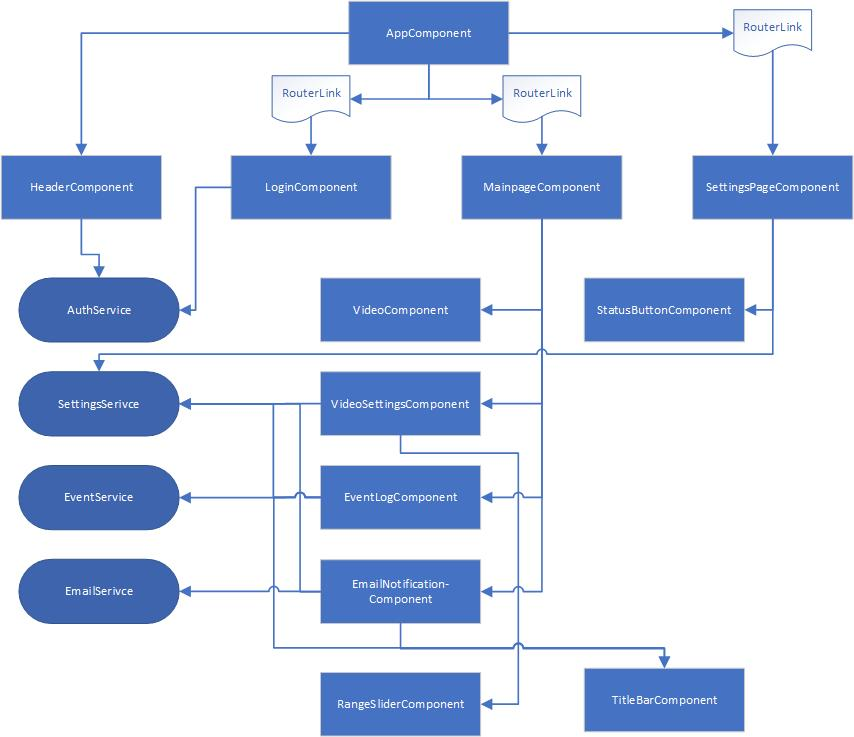
\includegraphics[]{content/pictures/KomponentenServiceDiagramm.jpg}
	\caption{Komponenten-Service-Diagramm zum Front-End}
	\label{fig:komponenten_service_diagramm}
\end{figure}
\chapter{Back-End}
Für die Entwicklung des Backends standen C++ und Python im Raum. Auf Empfehlung unseres Betreuers hin und aufgrund der einfachen Implementierung einiger Beispiele entschieden wir uns für die Entwicklung in Python.
\section{Konzept}
\section{Verwendete Open-Source Bibliotheken}
\subsection{OpenCV}
Bei OpenCV (Open Source Computer Vision Library) handelt es sich um eine Bibliothek zur Verarbeitung und Bearbeitung von Bildern und Video-Formaten. OpenCV wurde in C/C++ entwickelt und unterliegt derzeit einer Lizenz, die eine kostenlose Nutzung für akademische als auch kommerzielle Zwecke ermöglicht. Die Bibliothek unterstützt nicht nur herkömmliche Betriebssysteme wie Windows, Linux und Max OS, sondern auch Mobile Betriebssysteme wie iOS und Android. OpenCV wurde so entwickelt, dass es effizient in Echtzeitsystemen genutzt werden kann. In unserem Projekt werden wir für die Bearbeitung des Video-Streams mehrere Funktionalitäten der Bibliothek aufgreifen und verwenden.
\subsection{Numpy}
Bei NumPy handelt es sich um eine Python-exklusive Bibliothek. Diese wurde entwickelt, um mathematische Funktionen anzuwenden. Der Schwerpunkt hierbei liegt ins besonders auf Matrizen. Auch Numpy unterliegt der gleichen Lizenz wie OpenCV und erlaubt daher eine kostenlose Nutzung. In unserem System benötigen wir Numpy um ein paar Operationen auf unsere Bilder anzuwenden, oder auch um exemplarisch Bilder zu erstellen.
\section{Bildverarbeitungsprozess}
Um eine Bewegung aus mehreren Bildern erkennen zu können, reicht es normalerweise aus, die jeweiligen Pixelpositionen voneinander zu subtrahieren. Hat man an diesem Punkt noch weiße bzw. farbige Pixel, kann man davon ausgehen, dass es einen Unterschied gibt und daher auch eine Bewegung vorhanden ist. Da wir nun die Bewegungserkennungen einer Kamera umsetzen sollen, kann man nicht so simpel vorgehen. Es gibt mehrere kleinere Aspekte die beachtet werden können und es gibt auch keine einfache Lösung für einige Probleme. Im Laufe dieses Kapitels werden einige Probleme beleuchtet sowie Lösungen für diese aufgeführt, sofern umsetzbar.

\begin{figure}[ht]
	\flushright
	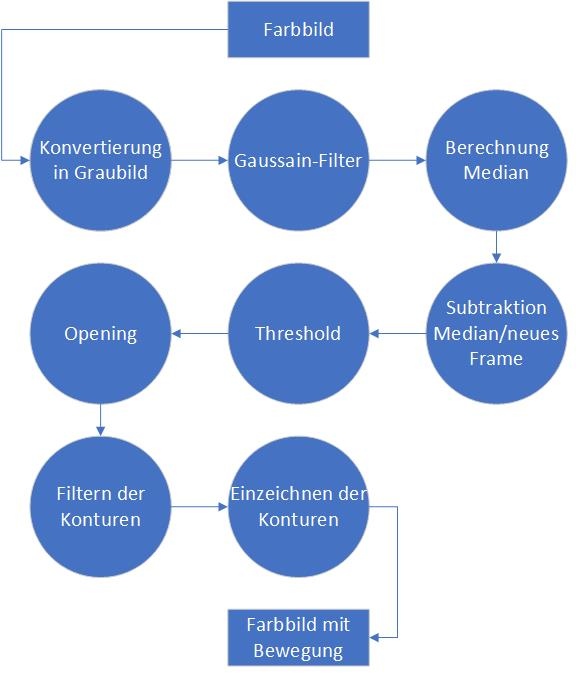
\includegraphics[]{content/pictures/Bildverarbeitung.jpg}
	\caption{Ablaufdiagramm der Bildverarbeitung}
\end{figure}

In dem Ablaufdiagramm kann man die Vorgehensweise unserer Bildverarbeitung sehen. Der erste Schritt beinhaltet die Konvertierung eines Farbwertbildes in ein Grauwertbild. Diese kann mit Hilfe von OpenCV leicht umgesetzt werden. Somit muss man sich keine Gedanken um den Datentyp des Bildes machen. Der Sinn hinter dieser Konvertierung bezieht sich stark auf die Performanz der kommenden Operationen, welche für die Bewegungserkennung notwendig sind. Würden wir alle Operationen mit einem Farbwertbild durchführen, hätten wir mindestens eine dreimal längere Laufzeit für die Bildverarbeitung.
Als nächsten Schritt entfernen wir das Rauschen aus dem Grauwertbild. Bei Rauschen in einem Bild handelt es sich um Pixelfehler die Werte enthalten, die dem eigentlichen Farbschema widersprechen. Diese entstehen meist direkt durch das Aufnahmegerät. Mithilfe des in OpenCV gebotenen Gaussain-Filters können diese bereinigt werden. Hierbei werden die umliegenden Pixel angeschaut und anhand denen entschieden, welchen Wert er erhalten wird. Sprich liegt der Pixel in einer dunklen grauen Fläche wird auch der Pixelwert den entsprechenden Grauwert erhalten.
Da wir nun das neue Bild vorbereitet haben, benötigen wir noch das vorherige Bild für den Vergleich. In unserem Fall berechnen wir Pixelweise den Median aus den letzten 15 Bildern. Durch dieses Vorgehen sollen kleinere Bewegungen von der Bewegungserkennung ignoriert werden. Für das Speichern der Bilder nutzen wir eine zyklische Liste, die das älteste Objekt beim überschreiten der maximalen Anzahl entfernt. Für die Berechnung des Medians bietet OpenCV leider keine Funktion. Daher greifen wir auf die Bibliothek NumPy zurück. Diese ermöglicht uns sowohl die Addition als auch das Berechnen des Medians. Gibt es keinen Fehler bei der Berechnung wird uns das berechnete Bild zurückgegeben, ansonsten erhalten wir das zuletzt hinzugefügte Bild zurück.
Haben wir nun das Median-Bild und das letzte Bild, können wir diese voneinander subtrahieren. Somit haben wir die Unterschiede aus den letzten Bildern. Die Subtraktion können wir direkt mit OpenCV ausführen.
Als Ergebnis der Subtraktion erhalten wir ein Bild mit unterschiedlichen Grauwerten. Wenn Grauwerte voneinander abgezogen werden, kann es sein, dass ähnliche Grauwerte trotzdem einen Grauwert größer als „0“ zurückgeben. Für uns spielen aber größere Änderungen eine Rolle. Um die niedrigen Grauwerte zu filtern, kann ein Threshold angewandt werden. Durch die Threshold-Funktion von OpenCV ist es uns möglich die Grauwerte mit einer Grenze in Schwarz und Weiß aufzuteilen.  Sprich alle Grauwerte  bis Beispielsweise dem Wert von 30 werden zu schwarz und alle höheren Grauwerte werden weiß.
Da wir kleine Bewegungen nicht als Bewegung zählen lassen wollen, müssen wir kleine Bereiche vorher entfernen. Durch die sogenannte Opening-Operation können kleine Bereiche gefiltert werden. Hierbei werden zuerst alle Bereiche erodiert und die übriggebliebenen Bereiche werden dilatiert. Dadurch bleiben die größeren Bereiche bestehen und kleine Bereiche werden entfernt. OpenCV bietet für die Erosion und Dilatation separate Funktionen an, die sich leicht verwenden lassen.
Als letzten Schritt Extrahieren wir, falls vorhanden, übrig gebliebene Konturen. Gibt es eine Kontur, gab es auch eine Bewegung, und die Pixelkoordinaten der Konturen werden in das Farbwertbild übernommen, um die Bewegung kenntlich zu machen und gegebenen falls werden Empfänger per E-Mail benachrichtigt.
\section{Performanceprobleme durch GIL}
Bei der Berechnung des Medians könnten sinnvoll mehrere Kerne benutzt werden. Dies müsste in Python jedoch über Umwege von Hand gemacht werden, da Multithreading durch den Global Interpreter Lock auf einen Kern beschränkt ist. Bei einem Versuch, bei dem für die Berechnung die Bilder in vier Teile aufgeteilt und eigene Prozesse erstellt wurden, erhöhte sich die Berechnungszeit sogar. Aufgrund des engen Zeitplans konnte dem Versuch der Performanceverbesserung nicht weiter nachgegangen werden.
\section{Zusätzliche Features}
\subsection{Video, Log und Thumbnail}
Es gibt mehrere Aspekte die wichtig für die Bildverarbeitung sind. Da wir über das Backend die Bilder für das Frontend zu Verfügung stellen und auch das Video erstellen, muss einiges in dieser Hinsicht beachtet werden. Zu Beginn haben wir sofort Video, Log und Thumbnail bei der ersten Bewegungserkennung zu Verfügung gestellt. Dies hatte zur Folge, dass beim Aktivieren des Videos die Aufnahme nicht fertiggestellt wird. Und kein Video angezeigt wird. Um dies zu umgehen, werden Video, Log und Thumbnail nur beim Abschluss der Bewegungssequenz weitergeleitet und das Thumbnail kann ein Bild mitten in der Bewegung darstellen.
\subsection{FPS-Berechnung}
OpenCV bietet eine Schnittstelle zum Erstellen von Videos. Hierbei muss vorab eine feste FPS (Frames Per Second) angegeben werden. Während den Tests ist uns aufgefallen, dass das Backend je nach System unterschiedlich schnell arbeitet. Zusätzlich dazu ist die Geschwindigkeit des Videos durch eine falsche Bearbeitungsrate verzerrt. Um dies zu vermeiden, berechnen wir die durchschnittliche FPS zur Laufzeit. Die ersten hundert benötigten Zeiten werden in einer Liste abgespeichert und am Schluss dividiert. Anhand dieses Wertes erhalten wir einen guten Wert, der auch das Video in einer angemessenen Geschwindigkeit darstellt.
\subsection{Maximale Cliplänge}
Um eine maximale Cliplänge gewährleisten zu können muss die Bearbeitungsrate aufgegriffen werden. Wurden genug Bilder gesammelt (FPS x maximale Cliplänge in Sekunden) wird das Video abgebrochen und eine neue Aufnahme wird gegebenenfalls gestartet.
\subsection{Wait for Motion-end}
Wurde gerade eine Bewegung erkannt und die Bewegungen haben aufgehört, wartet die Bearbeitung noch einen Moment ab, ob nicht doch noch eine Bewegung auftaucht. Dadurch wird die Aufnahme nicht direkt beendet, wenn keine Bewegung mehr erkannt wird und ein eventuell kurzer Aussetzer der Bewegung wird ignoriert.
\section{Datenhaltung und Speicherung}
Für die Datenhaltung wurde ein Singleton-Objekt mit den verschiedenen zu teilenden Daten erstellt. Um die Integrität der Daten zu gewährleisten musste darauf geachtet werden, dass keine Zugriffe gleichzeitig auf die jeweiligen Daten
gemacht werden können. Hierfür wurden Locks für die jeweiligen Datenobjekte erstellt.\\
Bei der Erstellung eines Backups dürfen ebenfalls keine Änderungen vorgenommen werden, weshalb alle Locks gesperrt werden müssen.\\
Die Daten müssen für die Anfrage passend zurückgegeben werden.
Damit die Daten nach dem Beenden des Programms noch vorhanden sind, sollten diese gespeichert werden. Da die Daten für die Kommunikation in JSON serialisiert werden müssen, wird auch für das Speichern ein JSONEncoder verwendet. Da die zu speichernden Attribute
der Objekte bereits serialisierbar sind, musste kein eigener Encoder geschrieben werden. Für die Decodierung musste jedoch eine Funktion geschrieben werden, welche die Art der Objekte anhand eines Keys prüft und aus den JSON-Daten wieder Objekte erstellt.
Es gibt drei JSON-Dateien mit denen die Emails, Logs sowie Einstellungen gespeichert werden.
\section{Mailclient}
Ein wesentlicher Teil eines Überwachungssystems ist die Benachrichtigung wie z.B. per Email.
Hierfür haben wir mit Hilfe der umfrangreichen Standardbibliothek in Python einen SMTP-Client erstellt.
Der Mailclient soll zum einen den Benutzer benachrichtigen, wenn eine Bewegung erkannt wurde und zum anderen wenn der maximal zu nutzende Speicher belegt ist.
Beim Start des Backends werden Login und Passwort abgefragt. Für Testzwecke wurde der Anbieter auf unseren verwendeten Provider vorbelegt.
\section{Webserver}
Für die Kommunikation mit dem Frontend sollte eine REST-Schnittstelle definiert werden. Hierzu wurde zuerst mit einem in den Standardbibliotheken verfügbaren HttpServer experimentiert,
welcher jedoch zu minimalisisch und dadurch für die Anwendung ungeeignet war. Anschließend wurde ein Flask-Webserver verwendet, bei welchem recht einfach über das Web Server Gateway Interface die Ressourcen definiert,
und auf diese Ressourcen bestimmte Funktionen registriert werden können. Am einfachsten ginge das mit Annotationen, wenn der Webserver als eigenes Programm läuft. Dies war in unserem Szenario jedoch nicht gegeben, weshalb der Webserver als Klasse definiert und die Pfade innerhalb des Konstruktors hinzugefügt wurden.\\
Der Webserver holt sich durch Anfragen die Daten vom Singleton-Objekt und sendet regelmäßig das aktuelle JPEG für den Videostream.
Allerdings gilt zu beachten, dass der von uns verwendete Webserver nicht für Produktivsysteme gedacht ist.

\section{Videoquelle}
\subsection{Voraussetzung}
Als Videoquelle bieten die meisten IP-Kameras die Bilder als MJPEG oder RTSP-Stream an.\\
Beide Formate werden durch OpenCV und somit durch unsere Anwendung unterstützt.
Ebenso kann OpenCV auch Videodateien unterschiedlicher Formate wie z.B. mp4 oder webm abspielen.
Von einer Youtube-Url kann jedoch nicht gestreamt werden, da Youtube nicht das File direkt zur Verfügung stellt.\\
Der Stream sollte mindestens 15 FPS zur Verfügung stellen, da wir somit auch den Median über den Zeitraum von etwa. einer Sekunde bilden. Wenn der Stream weniger Bilder sendet, wird der Median über einen längeren Zeitraum gebildet und somit ändert sich das Verhalten der Bilderkennung.

\subsection{Auflösung}
Aufgrund der o.g. Performanceprobleme ist die Verwendung einer höheren Auflösung ein großes Problem.\\ Für die Verwendung einer einfachen Bewegungserkennung reicht die Auflösung von 640x368 aus, jedoch erreichen wir selbst hierbei je nach Rechner nur ca. 20 FPS.
\chapter{Tests}
Diese Testdokumentation wurde erstellt, um die Herangehensweise, Durchführung sowie die Ergebnisse unseres Testprozesses festzuhalten.

\section{Testplan}

\subsection{Ziele}
Ziel unseres Testprozesses ist es garantieren zu können, dass die in diesem Projekt geschaffene Software unter den von uns festgelegten Vorraussetzungen annähernd bis vollständig fehlerfrei und mit möglichst guter Performance betrieben werden kann. Auffälligkeiten sowie nach dem Testprozess bekannte und unbehobene Fehler sollen am Ende des Testprozesses dokumentiert sein.

\subsection{Rahmenbedingungen}
Grundsätzlich wurde während der Entwicklung der Anwendung stets darauf geachtet, dass die jeweils neu implementierten Features einwandfrei funktionieren und auch, dass durch die Implementierung jener Features keine der zuvor vorhandenen Teile beschädigt werden. Dennoch haben wir in unserer Projektplanung eine gesonderte Testphase geplant, bei der wir im Zeitraum von zwei Wochen alle nötigen Schritte abschließen möchten, um die von uns erstellte Anwendung ausgiebig zu testen.



 

\subsection{Teststrategie}
Um unser Testziel zu erreichen greifen wir auf verschiedene Testmethoden zurück. Da die Testphase sowohl durch einen kurzen Zeitraum, als auch die Anzahl der Tester eingeschränkt ist, müssen wir diese Ressourcen bestmöglich nutzen. Nach längeren Diskussionen innerhalb des Entwicklungsteams haben wir uns dazu entschlossen, auf eine Kombination von automatisierten Unit-Tests, manuellen System- und UI-Tests, sowie Last-Test zu setzen. Auf diese Weise decken wir beim Testen nicht nur funktionale sondern auch nichtfunktionale Anforderungen der Software ab.

Welche Methodik bei den einzelnen Teilen der Anwendung verwendet wurde wird in der folgenden Tabelle dargestellt.

\begin{table}[]
	\begin{tabular}{|l|l|l|}
		\cline{1-2}
		\textbf{Testobjekt} & \textbf{Art des Testens} \\ \cline{1-2}
		Front-End           & \begin{tabular}[c]{@{}l@{}}Unit-Tests,\\ Manuelle Tests\end{tabular} \\ \cline{1-2}
		Back-End            & \begin{tabular}[c]{@{}l@{}}Unit-Tests.\\ Manuelle Tests\end{tabular} \\ \cline{1-2}
		Gesamtsystem        & Manuelle Tests \\ \cline{1-2}
	\end{tabular}
\end{table}

Trotz dessen, dass wir eine eigene Testphase geplant haben, ist es uns wichtig über den gesamten Entwicklungsprozess der Software für eine stets einwandfrei lauffähige Anwendung zu sorgen. Dies entspricht nicht nur unserem agilen Softwareentwicklungsprozess nach Scrum, sondern erleichtert auch die gemeinsame Arbeit durch mehrere Entwickler jeweils an Front-End sowie Back-End. Um dies gewährleisten zu können, haben wir abseits der Testphase jedes neu implementierte Feature sowie die Auswirkungen der Implementierung auf den Rest der Anwendung manuell getestet.

\section{Testen des Front-Ends}

\subsection{Unit-Tests}
Bei unserem Front-End sind wir zu dem Schluss gekommen, dass ein automatisiertes Testen nur bedingt sinnvoll ist. Ein großer Teil der Implementierungen dort bezieht sich rein auf die Darstellung der vom Back-End erhaltenen Daten im Webbrowser, oder um das Beschaffen und Versenden eben dieser Daten. Ein automatiertes Testen der Weboberfläche ist dabei überproportional aufwändig und in unserem Falle in den meisten Fällen nicht sinnvoll, da es sich vor allem um statische Inhalte oder um Video- beziehungsweise Bildinhalte handelt. Außerdem muss beim Testen einer Weboberfläche auf Faktoren wie Browserkompatibilität geachtet werden, was durch manuelles Testen besser umsetzbar ist. Nichts desto trotz wurde für jede Komponente des Front-Ends ein eigener Unit-Test erstellt, der die vollständige Erzeugung eben dieser Komponente simuliert und Testet. Dabei werden für die Komponente erforderliche Abhängigkeiten durch Mock-Objekte ersetzt, um ein unabhängiges Testen zu ermöglichen.

Standardgemäß verwenden wir beim automatisierten Testen unseres Angular-Front-Ends das Testframework Karma. Dieses ist bereits beim Erzeugen eines neuen Angular-Projektes per Angular-\acs{CLI} integriert und vorkonfiguriert. 

\subsubsection{Ausführen der Unit-Tests}
Nachdem das Projekt korrekt auf die in 23123 Dargestellte Art und Weise installiert wurde und lauffähig ist, können die automatisierten Tests durch das Aufrufen eines Konsolenbefehls gestartet werden. Dazu muss im Projektordner ein Terminal geöffnet werden und der Befehl "ng test" ausgeführt werden.

\subsubsection{Ergebnisse der Unit-Tests}
HIER SCREENSHOT VON UNITTEST ERGEBNISSEN EINFÜGEN


\subsection{Manuelle Tests}
Beim manuellen testen handelt es sich um einen Testprozess, bei dem der Tester ohne die Verwendung von Automatisierungstools vorgeht. Dabei können durch die systematische Verwendung der Software und das Nutzen von Diagnosetools oft Fehler aufgedeckt werden, die etwa bei Unit-Tests häufig nicht gefunden werden. Insbesondere Benutzeroberflächen können auf diese Weise unkompliziert getestet werden.

Im folgenden wird tabellarisch festgehalten, welche Aktionen getestet wurden und von welcher Ausgangssituation aus getestet wurde. Alle Tests wurden in den beiden Browsern Google Chrome (64-Bit Version 71.0.3578.98 Offizieller Build) und Mozilla Firefox (64-Bit Version 63.0.1 Offizieller Build) auf einem mit Windows 10 betriebenem Laptop mit einer Auflösung von 1920x1080 durchgeführt. 

\subsubsection{Ergebnisse der Manuellen Tests}
Vorraussetzung für alle Tests ist selbsterklärend, dass Front-End sowie Back-End korrekt installiert und gestartet sind.

\begin{longtable}{| p{.02\textwidth} | p{.06\textwidth} | p{.20\textwidth} | p{.20\textwidth} | p{.20\textwidth} | p{.07\textwidth} | p{.07\textwidth} |}
	\hline
	
	\textbf{\#} & \textbf{Kom-po-nen-te} & \textbf{Vorraussetz-ungen} & \textbf{Aktion} & \textbf{Erwartetes Ergebnis} & \textbf{OK in Chrome} & \textbf{OK in Firefox} \\ \hline
	
	1 & Login & Der Anwender befindet sich auf der Login-Seite und ist demnach nicht eingeloggt. & Der Anwender gibt beim Einloggen den richtigen Usernamen (user) und das richtige Passwort (geheim) ein. & Der Anwender wird auf die Hauptseite der Anwendung weitergeleitet und ist	korrekt eingeloggt. & X & X \\ \hline
	
	2 & Login & Der Anwender befindet sich auf der Login-Seite und ist demnach nicht
	eingeloggt. & Der Anwender gibt beim
	Einloggen einen falschen Usernamen (Verwendet: test) und das richtige Passwort (geheim) ein. & Rechts neben dem Login-Button erscheint eine Nachricht (Login failed) in roter Schrift. & X & X \\ \hline
	
	3 & Login & Der Anwender befindet sich auf der Login-Seite und ist demnach nicht eingeloggt. & Der Anwender gibt beim
	Einloggen den richtigen Usernamen (user) und ein falsches Passwort ein. (Verwendet: test) & Rechts neben dem Login-Button  erscheint eine Nachricht (Login failed) in roter Schrift. & X & X \\ \hline
	
	4 & Login & Der Anwender befindet sich auf der Login-Seite	und ist demnach nicht
	eingeloggt. & Der Anwender gibt beim Einloggen sowohl einen falschen Usernamen (Verwendet: test1) als auch ein falsches Passwort (Verwendet: test2) ein. & Rechts neben dem Login-Button erscheint eine Nachricht (Login failed) in roter Schrift. & X & X \\ \hline
	
	5 & Login & Der Anwender befindet sich auf der Login-Seite und ist demnach nicht eingeloggt. & Der Anwender gibt beim Einloggen einen falschen Usernamen (Verwendet: test) und das richtige Passwort (geheim) ein. & Zwischen dem Absenden der Logindaten und dem Empfangen einer Antwort durch das Back-End wird rechts neben dem Login-Button eine Ladeanimation angezeigt. & X & X \\ \hline
	
	6 & Login & Der Anwender befindet sich auf der Login-Seite und ist demnach nicht eingeloggt. & Der Anwender gibt beim Einloggen den richtigen Usernamen (user) und das richtige Passwort (geheim) ein. & Zwischen dem Absenden	der Logindaten und dem Empfangen einer Antwort
	durch das Back-End wird	rechts neben dem Login-
	Button eine Ladeanimation angezeigt.  & X & X \\ \hline
	
	7 & Header & Der Anwender befindet sich auf der Login-Seite
	und ist demnach nicht eingeloggt. & Der Anwender klickt auf das
	PIPCO-Logo auf der linken Seite des Headers. & Die Webseite wird neu geladen. & X & X \\ \hline
	
	8 & Header & Der Anwender befindet sich auf der Settings-Seite und ist demnach	bereits eingeloggt. & Der Anwender klickt auf das PIPCO-Logo auf der linken Seite des Headers. & Die Webseite wird neu geladen. Der Anwender ist
	nicht länger eingeloggt und	wird daher auf die Login-Seite weitergeleitet. & X & X \\ \hline
	
	9 & Header & & Der Anwender hovert mit dem Cursor über das PIPCO-Logo auf der linken Siete des Headers. & Ein Tooltip (Refresh Page) wird neben dem Cursor angezeigt. Der Cursor ändert sein Styling zu Pointer. & X & X \\ \hline
	
	10 & Header & Der Anwender ist korrekt eingeloggt und befindet sich auf der Hauptseite & & Auf der rechten Seite des headers befinden sich ein Settings-Button sowie ein Logout-Button (in dieser Reihenfolge) & X & X \\ \hline
	
	11 & Header & Der Anwender ist korrekt eingeloggt und befindet sich auf der Hauptseite. & Der Anwender hovert mit dem Cursor über den Settings-Button auf der rechten Seite des Headers. & Ein Tooltip (Settings) wird neben dem Cursor angezeigt. Der Cursor ändert sein Styling zu Pointer. & X & X \\ \hline
	
	12 & Header & Der Anwender ist korrekt eingeloggt und befindet sich auf der Hauptseite. & Der Anwender hovert mit dem Cursor über den Logout-Button auf der rechten Seite des Headers. & Ein Tooltip (Logout) wird neben dem Cursor angezeigt. Der Cursor ändert sein Styling zu Pointer. & X & X \\ \hline
	
	13 & Header & Der Anwender ist korrekt eingeloggt und befinet sich auf der Hauptseite. & Der Anwender klickt auf den Settings-Button auf der rechten Seite des Headers. & Der Anwender wird auf die Settings-Seite weitergeleitet. & X & X \\ \hline

	14 & Header & Der Anwender ist korrekt eingeloggt und befinet sich auf der Hauptseite. & Der Anwender klickt auf den Logout-Button auf der rechten Seite des Headers. & Der Anwender wird korrekt ausgeloggt und auf die Login-Seite weitergeleitet. & X & X \\ \hline

	15 & Header & Der Anwender ist korrekt eingeloggt und befinet sich auf der Settings-Seite. & & Auf der rechten Seite des Headers befinden sich ein Home-Button sowie ein Logout-Button (in dieser Reihenfolge) & X & X \\ \hline
	
	16 & Header & Der Anwender ist korrekt eingeloggt und befindet sich auf der Settings-Seite. & Der Anwender klickt auf den Home-Button auf der rechten Seite des Headers. & Der Anwender wird auf die Hauptseite weitergeleitet & X & X \\ \hline
	
	17 & Header & Der Anwender ist korrekt eingeloggt und befindet sich auf der Settings-Seite. & Der Anwender klickt auf den Logout-Button auf der rechten Seite des Headers. & Settings-Button sowie Logout-Button im Header sind nicht mehr da. & X & X \\ \hline
	
	18 & Header & Der Anwender ist korrekt eingeloggt und befindet sich auf der Settings-Seite. & Der Anwender hovert mit dem Cursor über den Home-Button auf der rechten Seite des Headers. & Ein Tooltip (Home) wird neben dem Cursor angezeigt. Der Cursor ändert sein Styling zu Pointer. & X & X \\ \hline
	
	\caption{Manuelle Front-End-Tests}
	\label{tab:manuelle_front_end_tests}
\end{longtable}

\begin{longtable}{c} 
\centering
\resizebox{\textwidth}{!}{
\begin{tabular}{cllllcc}
	\hline
	\multicolumn{1}{|l|}{\textbf{\#}} & \multicolumn{1}{l|}{Komponente} & \multicolumn{1}{l|}{\textbf{Aktion}}                                                                                                                                                                              & \multicolumn{1}{l|}{\textbf{Voraussetzungen}}                                                                                                             & \multicolumn{1}{l|}{\textbf{Erwartetes Ergebnis}}                                                                                                                                                                                    & \multicolumn{1}{l|}{\textbf{\begin{tabular}[c]{@{}l@{}}Test in \\ Chrome \\ bestanden\end{tabular}}} & \multicolumn{1}{l|}{\textbf{\begin{tabular}[c]{@{}l@{}}Test in \\ Firefox \\ Bestanden\end{tabular}}} \\ \hline
	\multicolumn{1}{|c|}{1}           & \multicolumn{1}{l|}{Login}      & \multicolumn{1}{l|}{\begin{tabular}[c]{@{}l@{}}Der Anwender gibt beim\\ Einloggen den richtigen User-\\ namen (user) und das richtige\\ Passwort (geheim) ein.\end{tabular}}                                      & \multicolumn{1}{l|}{\begin{tabular}[c]{@{}l@{}}Der Anwender befindet\\ sich auf der Login-Seite\\ und ist demnach nicht\\ eingeloggt.\end{tabular}}       & \multicolumn{1}{l|}{\begin{tabular}[c]{@{}l@{}}Der Anwender wird auf die\\ Hauptseite der Anwendung\\ weitergeleitet und ist\\ korrekt eingeloggt.\end{tabular}}                                                                     & \multicolumn{1}{c|}{X}                                                                               & \multicolumn{1}{c|}{X}                                                                                \\ \hline
	\multicolumn{1}{|c|}{2}           & \multicolumn{1}{l|}{Login}      & \multicolumn{1}{l|}{\begin{tabular}[c]{@{}l@{}}Der Anwender gibt beim\\ Einloggen einen falschen User-\\ namen (Verwendet: test) und\\ das richtige Passwort (geheim)\\ ein.\end{tabular}}                        & \multicolumn{1}{l|}{\begin{tabular}[c]{@{}l@{}}Der Anwender befindet\\ sich auf der Login-Seite\\ und ist demnach nicht\\ eingeloggt.\end{tabular}}       & \multicolumn{1}{l|}{\begin{tabular}[c]{@{}l@{}}Rechts neben dem Login-\\ Button  erscheint eine \\ Nachricht (Login failed)\\ in roter Schrift.\end{tabular}}                                                                        & \multicolumn{1}{c|}{X}                                                                               & \multicolumn{1}{c|}{X}                                                                                \\ \hline
	\multicolumn{1}{|l|}{3}           & \multicolumn{1}{l|}{Login}      & \multicolumn{1}{l|}{\begin{tabular}[c]{@{}l@{}}Der Anwender gibt beim\\ Einloggen den richtigen User-\\ namen (user) und ein falsches\\ Passwort ein. (Verwendet: test)\end{tabular}}                             & \multicolumn{1}{l|}{\begin{tabular}[c]{@{}l@{}}Der Anwender befindet\\ sich auf der Login-Seite\\ und ist demnach nicht\\ eingeloggt.\end{tabular}}       & \multicolumn{1}{l|}{\begin{tabular}[c]{@{}l@{}}Rechts neben dem Login-\\ Button  erscheint eine \\ Nachricht (Login failed)\\ in roter Schrift.\end{tabular}}                                                                        & \multicolumn{1}{c|}{X}                                                                               & \multicolumn{1}{c|}{X}                                                                                \\ \hline
	\multicolumn{1}{|c|}{4}           & \multicolumn{1}{l|}{Login}      & \multicolumn{1}{l|}{\begin{tabular}[c]{@{}l@{}}Der Anwender gibt beim\\ Einloggen sowohl einen\\ falschen Usernamen\\ (Verwendet: test1) als auch\\ ein falsches Passwort\\ (Verwendet: test2) ein.\end{tabular}} & \multicolumn{1}{l|}{\begin{tabular}[c]{@{}l@{}}Der Anwender befindet\\ sich auf der Login-Seite\\ und ist demnach nicht\\ eingeloggt.\end{tabular}}       & \multicolumn{1}{l|}{\begin{tabular}[c]{@{}l@{}}Rechts neben dem Login-\\ Button  erscheint eine \\ Nachricht (Login failed)\\ in roter Schrift.\end{tabular}}                                                                        & \multicolumn{1}{c|}{X}                                                                               & \multicolumn{1}{c|}{X}                                                                                \\ \hline
	\multicolumn{1}{|c|}{5}           & \multicolumn{1}{l|}{Login}      & \multicolumn{1}{l|}{\begin{tabular}[c]{@{}l@{}}Der Anwender gibt beim\\ Einloggen einen falschen User-\\ namen (Verwendet: test) und\\ das richtige Passwort (geheim)\\ ein.\end{tabular}}                        & \multicolumn{1}{l|}{\begin{tabular}[c]{@{}l@{}}Der Anwender befindet\\ sich auf der Login-Seite\\ und ist demnach nicht\\ eingeloggt.\end{tabular}}       & \multicolumn{1}{l|}{\begin{tabular}[c]{@{}l@{}}Zwischen dem Absenden\\ der Logindaten und dem\\ Empfangen einer Antwort\\ durch das Back-End wird\\ rechts neben dem Login-\\ Button eine Ladeanima-\\ tion angezeigt.\end{tabular}} & \multicolumn{1}{c|}{X}                                                                               & \multicolumn{1}{c|}{X}                                                                                \\ \hline
	\multicolumn{1}{|c|}{6}           & \multicolumn{1}{l|}{Login}      & \multicolumn{1}{l|}{\begin{tabular}[c]{@{}l@{}}Der Anwender gibt beim\\ Einloggen den richtigen User-\\ namen (user) und das richtige\\ Passwort (geheim) ein.\end{tabular}}                                      & \multicolumn{1}{l|}{\begin{tabular}[c]{@{}l@{}}Der Anwender befindet\\ sich auf der Login-Seite\\ und ist demnach nicht\\ eingeloggt.\end{tabular}}       & \multicolumn{1}{l|}{\begin{tabular}[c]{@{}l@{}}Zwischen dem Absenden\\ der Logindaten und dem\\ Empfangen einer Antwort\\ durch das Back-End wird\\ rechts neben dem Login-\\ Button eine Ladeanima-\\ tion angezeigt.\end{tabular}} & \multicolumn{1}{c|}{X}                                                                               & \multicolumn{1}{c|}{X}                                                                                \\ \hline
	\multicolumn{1}{|c|}{7}           & \multicolumn{1}{l|}{Header}     & \multicolumn{1}{l|}{\begin{tabular}[c]{@{}l@{}}Der Anwender klickt auf das\\ PIPCO-Logo auf der linken\\ Seite des Headers.\end{tabular}}                                                                         & \multicolumn{1}{l|}{\begin{tabular}[c]{@{}l@{}}Der Anwender befindet\\ sich auf der Login-Seite\\ und ist demnach nicht\\ eingeloggt.\end{tabular}}       & \multicolumn{1}{l|}{\begin{tabular}[c]{@{}l@{}}Die Webseite wird neu\\ geladen.\end{tabular}}                                                                                                                                        & \multicolumn{1}{c|}{X}                                                                               & \multicolumn{1}{c|}{X}                                                                                \\ \hline
	\multicolumn{1}{|c|}{8}           & \multicolumn{1}{l|}{Header}     & \multicolumn{1}{l|}{\begin{tabular}[c]{@{}l@{}}Der Anwender klickt auf das\\ PIPCO-Logo auf der linken\\ Seite des Headers.\end{tabular}}                                                                         & \multicolumn{1}{l|}{\begin{tabular}[c]{@{}l@{}}Der Anwender befindet\\ sich auf der Settings-\\ Seite und ist demnach\\ bereits eingeloggt.\end{tabular}} & \multicolumn{1}{l|}{\begin{tabular}[c]{@{}l@{}}Die Webseite wird neu\\ geladen. Der Anwender ist\\ nicht länger eingeloggt und\\ wird daher auf die Login-\\ Seite weitergeleitet.\end{tabular}}                                     & \multicolumn{1}{c|}{X}                                                                               & \multicolumn{1}{c|}{X}                                                                                \\ \hline
	\multicolumn{1}{|c|}{9}           & \multicolumn{1}{l|}{Header}     & \multicolumn{1}{l|}{\begin{tabular}[c]{@{}l@{}}Der Anwender hovert mit dem\\ Cursor über das PIPCO-Logo\\ auf der linken Seite des\\ Headers.\end{tabular}}                                                       & \multicolumn{1}{l|}{}                                                                                                                                     & \multicolumn{1}{l|}{\begin{tabular}[c]{@{}l@{}}Ein Tooltip (Refresh Page)\\ wird neben dem Cursor\\ angezeigt. Der Cursor \\ ändert sein Styling zu\\ Pointer.\end{tabular}}                                                         & \multicolumn{1}{c|}{X}                                                                               & \multicolumn{1}{c|}{X}                                                                                \\ \hline
	\multicolumn{1}{|c|}{10}          & \multicolumn{1}{l|}{Header}     & \multicolumn{1}{l|}{}                                                                                                                                                                                             & \multicolumn{1}{l|}{\begin{tabular}[c]{@{}l@{}}Der Anwender ist korrekt\\ eingeloggt und befindet \\ sich auf der Hauptseite.\end{tabular}}               & \multicolumn{1}{l|}{\begin{tabular}[c]{@{}l@{}}Auf der rechten Seite des\\ Headers befinden sich ein\\ Settings-Button sowie ein\\ Logout-Button (in dieser\\ Reihenfolge).\end{tabular}}                                            & \multicolumn{1}{c|}{X}                                                                               & \multicolumn{1}{c|}{X}                                                                                \\ \hline
	\multicolumn{1}{|c|}{11}          & \multicolumn{1}{l|}{Header}     & \multicolumn{1}{l|}{\begin{tabular}[c]{@{}l@{}}Der Anwender hovert mit dem\\ Cursor über den Settings-\\ Button auf der rechten Seite \\ des Headers.\end{tabular}}                                               & \multicolumn{1}{l|}{\begin{tabular}[c]{@{}l@{}}Der Anwender ist korrekt\\ eingeloggt und befindet\\ sich auf der Hauptseite.\end{tabular}}                & \multicolumn{1}{l|}{\begin{tabular}[c]{@{}l@{}}Ein Tooltip (Refresh Page)\\ wird neben dem Cursor\\ angezeigt. Der Cursor \\ ändert sein Styling zu\\ Pointer.\end{tabular}}                                                         & \multicolumn{1}{c|}{X}                                                                               & \multicolumn{1}{c|}{X}                                                                                \\ \hline
	\multicolumn{1}{|l|}{12}          & \multicolumn{1}{l|}{Header}     & \multicolumn{1}{l|}{\begin{tabular}[c]{@{}l@{}}Der Anwender hovert mit dem\\ Cursor über den Logout-\\ Button auf der rechten Seite \\ des Headers.\end{tabular}}                                                 & \multicolumn{1}{l|}{\begin{tabular}[c]{@{}l@{}}Der Anwender ist korrekt\\ eingeloggt und befindet\\ sich auf der Hauptseite.\end{tabular}}                & \multicolumn{1}{l|}{\begin{tabular}[c]{@{}l@{}}Ein Tooltip (Logout)\\ wird neben dem Cursor\\ angezeigt. Der Cursor \\ ändert sein Styling zu\\ Pointer.\end{tabular}}                                                               & \multicolumn{1}{c|}{X}                                                                               & \multicolumn{1}{c|}{X}                                                                                \\ \hline
	\multicolumn{1}{|c|}{13}          & \multicolumn{1}{l|}{Header}     & \multicolumn{1}{l|}{\begin{tabular}[c]{@{}l@{}}Der Anwender klickt auf den\\ Settings-Button auf der rechten\\ Seite des Headers.\end{tabular}}                                                                   & \multicolumn{1}{l|}{\begin{tabular}[c]{@{}l@{}}Der Anwender ist korrekt\\ eingeloggt und befindet\\ sich auf der Hauptseite.\end{tabular}}                & \multicolumn{1}{l|}{\begin{tabular}[c]{@{}l@{}}Der Anwender wird auf die\\ Settings-Seite\\ weitergeleitet.\end{tabular}}                                                                                                            & \multicolumn{1}{c|}{X}                                                                               & \multicolumn{1}{c|}{X}                                                                                \\ \hline
	\multicolumn{1}{|c|}{14}          & \multicolumn{1}{l|}{Header}     & \multicolumn{1}{l|}{\begin{tabular}[c]{@{}l@{}}Der Anwender klickt auf den\\ Logout-Button auf der rechten\\ Seite des Headers.\end{tabular}}                                                                     & \multicolumn{1}{l|}{\begin{tabular}[c]{@{}l@{}}Der Anwender ist korrekt\\ eingeloggt und befindet\\ sich auf der Hauptseite.\end{tabular}}                & \multicolumn{1}{l|}{\begin{tabular}[c]{@{}l@{}}Der Anwender wird korrekt\\ ausgeloggt und auf die\\ Login-Seite weitergeleitet.\end{tabular}}                                                                                        & \multicolumn{1}{c|}{X}                                                                               & \multicolumn{1}{c|}{X}                                                                                \\ \hline
	\multicolumn{1}{|c|}{15}          & \multicolumn{1}{l|}{Header}     & \multicolumn{1}{l|}{}                                                                                                                                                                                             & \multicolumn{1}{l|}{\begin{tabular}[c]{@{}l@{}}Der Anwender ist korrekt\\ eingeloggt und befindet\\ sich auf der \\ Settings-Seite.\end{tabular}}         & \multicolumn{1}{l|}{\begin{tabular}[c]{@{}l@{}}Auf der rechten Seite des\\ Headers befinden sich ein\\ Home-Button sowie ein\\ Logout-Button (in dieser\\ Reihenfolge).\end{tabular}}                                                & \multicolumn{1}{c|}{X}                                                                               & \multicolumn{1}{c|}{X}                                                                                \\ \hline
	\multicolumn{1}{|c|}{16}          & \multicolumn{1}{l|}{Header}     & \multicolumn{1}{l|}{\begin{tabular}[c]{@{}l@{}}Der Anwender klickt auf den\\ Home-Button auf der rechten\\ Seite des Headers.\end{tabular}}                                                                       & \multicolumn{1}{l|}{\begin{tabular}[c]{@{}l@{}}Der Anwender ist korrekt\\ eingeloggt und befindet\\ sich auf der\\ Settings-Seite.\end{tabular}}          & \multicolumn{1}{l|}{\begin{tabular}[c]{@{}l@{}}Der Anwender wird auf\\ die Hauptseite\\ weitergeleitet..\end{tabular}}                                                                                                               & \multicolumn{1}{c|}{X}                                                                               & \multicolumn{1}{c|}{X}                                                                                \\ \hline
	\multicolumn{1}{|c|}{17}          & \multicolumn{1}{l|}{Header}     & \multicolumn{1}{l|}{\begin{tabular}[c]{@{}l@{}}Der Anwender klickt auf den\\ Logout-Button auf der rechten\\ Seite des Headers.\end{tabular}}                                                                     & \multicolumn{1}{l|}{\begin{tabular}[c]{@{}l@{}}Der Anwender ist korrekt\\ eingeloggt und befindet\\ sich auf der Hauptseite.\end{tabular}}                & \multicolumn{1}{l|}{\begin{tabular}[c]{@{}l@{}}Settings-Button sowie\\ Logout-Button im Header\\ sind nicht mehr da.\end{tabular}}                                                                                                   & \multicolumn{1}{c|}{X}                                                                               & \multicolumn{1}{c|}{X}                                                                                \\ \hline
	\multicolumn{1}{|c|}{18}          & \multicolumn{1}{l|}{Header}     & \multicolumn{1}{l|}{\begin{tabular}[c]{@{}l@{}}Der Anwender hovert mit dem\\ Cursor über den Home-\\ Button auf der rechten Seite \\ des Headers.\end{tabular}}                                                   & \multicolumn{1}{l|}{\begin{tabular}[c]{@{}l@{}}Der Anwender ist korrekt\\ eingeloggt und befindet\\ sich auf der\\ Settings-Seite.\end{tabular}}          & \multicolumn{1}{l|}{\begin{tabular}[c]{@{}l@{}}Ein Tooltip (Home)\\ wird neben dem Cursor\\ angezeigt. Der Cursor \\ ändert sein Styling zu\\ Pointer.\end{tabular}}                                                                 & \multicolumn{1}{c|}{X}                                                                               & \multicolumn{1}{c|}{X}                                                                                \\ \hline
	\multicolumn{1}{|c|}{19}          & \multicolumn{1}{l|}{}           & \multicolumn{1}{l|}{}                                                                                                                                                                                             & \multicolumn{1}{l|}{}                                                                                                                                     & \multicolumn{1}{l|}{}                                                                                                                                                                                                                & \multicolumn{1}{c|}{}                                                                                & \multicolumn{1}{c|}{}                                                                                 \\ \hline
	\multicolumn{1}{|c|}{20}          & \multicolumn{1}{l|}{}           & \multicolumn{1}{l|}{}                                                                                                                                                                                             & \multicolumn{1}{l|}{}                                                                                                                                     & \multicolumn{1}{l|}{}                                                                                                                                                                                                                & \multicolumn{1}{c|}{}                                                                                & \multicolumn{1}{c|}{}                                                                                 \\ \hline
	\multicolumn{1}{|c|}{21}          & \multicolumn{1}{l|}{}           & \multicolumn{1}{l|}{}                                                                                                                                                                                             & \multicolumn{1}{l|}{}                                                                                                                                     & \multicolumn{1}{l|}{}                                                                                                                                                                                                                & \multicolumn{1}{c|}{}                                                                                & \multicolumn{1}{c|}{}                                                                                 \\ \hline
	\multicolumn{1}{|c|}{22}          & \multicolumn{1}{l|}{}           & \multicolumn{1}{l|}{}                                                                                                                                                                                             & \multicolumn{1}{l|}{}                                                                                                                                     & \multicolumn{1}{l|}{}                                                                                                                                                                                                                & \multicolumn{1}{c|}{}                                                                                & \multicolumn{1}{c|}{}                                                                                 \\ \hline
	\multicolumn{1}{|c|}{23}          & \multicolumn{1}{l|}{}           & \multicolumn{1}{l|}{}                                                                                                                                                                                             & \multicolumn{1}{l|}{}                                                                                                                                     & \multicolumn{1}{l|}{}                                                                                                                                                                                                                & \multicolumn{1}{c|}{}                                                                                & \multicolumn{1}{c|}{}                                                                                 \\ \hline
	\multicolumn{1}{l}{}              &                                 &                                                                                                                                                                                                                   &                                                                                                                                                           &                                                                                                                                                                                                                                      & \multicolumn{1}{l}{}                                                                                 & \multicolumn{1}{l}{}                                                                                  \\
	\multicolumn{1}{l}{}              &                                 &                                                                                                                                                                                                                   &                                                                                                                                                           &                                                                                                                                                                                                                                      & \multicolumn{1}{l}{}                                                                                 & \multicolumn{1}{l}{}                                                                                  \\
	\multicolumn{1}{l}{}              &                                 &                                                                                                                                                                                                                   &                                                                                                                                                           &                                                                                                                                                                                                                                      & \multicolumn{1}{l}{}                                                                                 & \multicolumn{1}{l}{}                                                                                  \\
	\multicolumn{1}{l}{}              &                                 &                                                                                                                                                                                                                   &                                                                                                                                                           &                                                                                                                                                                                                                                      & \multicolumn{1}{l}{}                                                                                 & \multicolumn{1}{l}{}                                                                                 
\end{tabular}}
\end{longtable}

\chapter{Installation}

\section{System}
Die Installationsanweisungen wurden auf einem Ubuntu Server der Version 18.10 durchgeführt.\\
Hierzu wurde ein bereits installiertes Image für VirtualBox von \\ \texttt{https://www.osboxes.org/ubuntu-server/} verwendet.
  
\section{Backend}
Für das Backend muss OpenCV, sowie der Flask-Webserver mit allen notwendigen Modulen installiert werden.
Die Lightweight Installation von OpenCV, welche einfach mit pip installiert werden kann, enthält nicht den passenden Encoder für mp4, weshalb der aktuelle Stand selbst geladen und compiliert werden muss.
Hierzu kann folgende Anleitung verwendet werden:\\
\texttt{https://www.pyimagesearch.com/2018/05/28/ubuntu-18-04-how-to-install-opencv/}
Zusätzlich zur Installation von OpenCV muss Flask mit pip installiert werden.
Hierzu muss wie in der Anleitung beschrieben .bashrc mit 
\begin{lstlisting}[frame=single]
source  ~/.bashrc
\end{lstlisting}
geladen werden.
Anschließend kann mit
\begin{lstlisting}[frame=single]
workon cv
\end{lstlisting} in der Virtuellen Python-Umgebung gearbeitet bzw. flask wie folgt installiert werden:
\begin{lstlisting}[frame=single]
pip install flask flask-cors
\end{lstlisting}
Nun muss nur noch das Repository ausgecheckt und ausgeführt werden.
\begin{lstlisting}[frame=single]
git clone https://github.com/PIPCO-1819/PIPCO-Backend
cd PIPCO-Backend
python Main.py
\end{lstlisting}

\section{Frontend}
Für das Frontend wird Node.js, npm, sowie Angular verwendet.
\begin{lstlisting}[frame=single]
apt-get install npm nodejs
sudo npm install -g npm@latest
sudo npm install -g @angular/cli
\end{lstlisting}
Repository auschecken und restliche dependencies installieren:
\begin{lstlisting}[frame=single]
git clone https://github.com/PIPCO-1819/PIPCO-Frontend.git
cd PIPCO-Frontend
npm install
\end{lstlisting}
Anschließend den Server wie folgt starten:
\begin{lstlisting}[frame=single]
ng serve --host 0.0.0.0
\end{lstlisting}

\section{Run on Startup}
start\_backend.sh in PIPCO-Backend
\begin{lstlisting}[frame=single]
#!/bin/sh
printf "<LOGIN>\n<PASSWORD>\n" | \
/home/osboxes/.virtualenvs/cv/bin/python Main.py
\end{lstlisting}

start\_frontend.sh in PIPCO-Frontend
\begin{lstlisting}[frame=single]
#!/bin/sh
printf "<LOGIN>\n<PASSWORD>\n" | \
/home/osboxes/.virtualenvs/cv/bin/python Main.py
\end{lstlisting}

start\_frontend.sh in PIPCO-Frontend
\begin{lstlisting}[frame=single]
#!/bin/sh
ng serve --host 0.0.0.0
\end{lstlisting}

start\_pipco.sh
\begin{lstlisting}[frame=single]
#!/bin/bash
screen -dmS frontend bash -c \
'cd /home/osboxes/PIPCO-Frontend; ./start_frontend.sh'
screen -dmS backend bash -c \
'cd /home/osboxes/PIPCO-Backend;. start_backend.sh'
\end{lstlisting}

rc.local bei Start des Systems ausführen
\begin{lstlisting}[frame=single]
printf '%s\n' '#!/bin/bash' 'exit 0' | sudo tee -a /etc/rc.local
sudo chmod +x /etc/rc.local
\end{lstlisting}
Skript zu rc.local hinzufügen
\begin{lstlisting}[frame=single]
...
/home/osboxes/start_pipco.sh
exit 0
\end{lstlisting}
\chapter{Ausblick}
Eine einfache Bewegungserkennung und Aufnahme der Bewegung wurde erfolgreich umgesetzt. Des weiteren können bereits einige Einstellungen vorgenommen werden. Jedoch bietet dieses Projekt noch viele Möglichkeiten.\\
Die Berechnung des Medians kann in Zukunft auf mehrere Prozesse aufgeteilt werden oder es findet sich eine Möglichkeit die Erkennung der Bewegung über mehrere Frames einfacher zu gestalten.
Mit einer besseren Performance könnten somit auch höhere Auflösungen verarbeitet werden.
Außerdem wäre es praktisch mehrere Kamerastreams mit Tags (z.B. Wohnzimmer) der Website hinzuzufügen zu können und bei einer erkannten Bewegung zusätzlich darüber benachrichtigt zu werden, von welcher Kamera diese Bewegung erkannt wurde. Hierfür müsste ein eigener Prozess für jede Bildverarbeitunsroutine gestartet werden, wobei dann für die Datenhaltung auch eine neue Lösung (IPC) gefunden werden müsste, da diese Prozesse keinen gemeinsamen Bereich im RAM verwenden.\\
Eine weitere Verbesserung wäre die Kommunikation über den Front-End-Server zu leiten, welcher dann vom Backend über Änderungen informiert wird und diese aktualisierten Informationen an den Client weitergibt. Somit wäre das Back-End entlastet und könnte nach außen unsichtbar gemacht werden. Der Login ist momentan außerdem durch die jetzige Implementierung mit etwas Javascript-Änderungen zu umgehen. Es wird lediglich Client-seitig die Antwort des Back-Ends überprüft.\\
Die Benachrichtung könnte man vielleicht auch etwas moderner gestalten. Hierbei wäre eine App oder eine Progressive Web App für eine Push-Benachrichtigung interessant.\\
Mit OpenCV könnte auch in Richtung des Deep Learnings gearbeitet werden und damit vielleicht z.B. das Haustier mittels Object Detection erkannt und somit als Bewegung ignoriert werden.
\chapter{Fazit}

% Schalgwortverzeichnis (Index)
%\printindex

% Literaturverzeichnis
\singlespacing
\bibliographystyle{alphadin}
\bibliography{bibtex}

% Eidesstattliche Erklärung
\chapter*{Eidesstattliche Erklärung\markboth{Eidesstattliche Erklärung}{}}
% Eintrag in das Inhaltsverzeichnis 
\addcontentsline{toc}{chapter}{Eidesstattliche Erklärung}

Ich versichere, dass ich die vorstehende Arbeit selbständig verfasst und hierzu
keine anderen als die angegebenen Hilfsmittel verwendet habe. Alle Stellen der Arbeit die 
wörtlich oder sinngemäß aus fremden Quellen entnommen wurden, sind als solche kenntlich gemacht.
\\
\\
Die Arbeit wurde bisher in gleicher oder ähnlicher Form in keinem anderen
Studiengang als Prüfungsleistung vorgelegt oder an anderer Stelle
veröffentlicht.
\\
\\
Ich bin mir bewusst, dass eine falsche Erklärung rechtliche Folgen haben kann.

\vspace*{1.5cm} \par
\line(1,0){200} \par
\docOrt, den  \docAbgabedatum ~~\docVorname~\docNachname

\appendix
% Hier können Anhaenge angefuegt werden

\end{document}      